% **************************************************************************************************************
% A Classic Thesis Style
% An Homage to The Elements of Typographic Style
%
% Copyright (C) 2012 Andr\'e Miede http://www.miede.de
%
% If you like the style then I would appreciate a postcard. My address
% can be found in the file ClassicThesis.pdf. A collection of the
% postcards I received so far is available online at
% http://postcards.miede.de
%
% License:
% This program is free software; you can redistribute it and/or modify
% it under the terms of the GNU General Public License as published by
% the Free Software Foundation; either version 2 of the License, or
% (at your option) any later version.
%
% This program is distributed in the hope that it will be useful,
% but WITHOUT ANY WARRANTY; without even the implied warranty of
% MERCHANTABILITY or FITNESS FOR A PARTICULAR PURPOSE.  See the
% GNU General Public License for more details.
%
% You should have received a copy of the GNU General Public License
% along with this program; see the file COPYING.  If not, write to
% the Free Software Foundation, Inc., 59 Temple Place - Suite 330,
% Boston, MA 02111-1307, USA.
%
% **************************************************************************************************************
% Note:
%    * You must not use "u etc. in strings/commands that will be spaced out (use \"u or real umlauts instead)
%    * New enumeration (small caps): \begin{aenumerate} \end{aenumerate}
%    * For margin notes: \marginpar or \graffito{}
%    * Do not use bold fonts in this style, it is designed around them
%    * Use tables as in the examples
%    * See classicthesis-preamble.sty for useful commands
% **************************************************************************************************************
% To Do:
%		 * [high] Check this out: http://www.golatex.de/koma-script-warnung-in-verbindung-mit-listings-package-t2058.html
%    * [medium] mathbb in section-titles/chapter-titles => disappears somehow in headlines!!!
% **************************************************************************************************************
%To compile: % DB
%
% pdflatex ClassicThesis.tex
% bibtex FrontBackmatter/Publication
% bibtex Chapters/Introduction
% bibtex Chapters/plasma_probe_physics
% bibtex Chapters/hardware
% bibtex Chapters/electronics_data_processing
% bibtex Chapters/compare_measurements
% bibtex Chapters/death_ray
% bibtex Chapters/ISP_space_charge
% bibtex Chapters/Ti_Te_SOL
% bibtex FrontBackmatter/sheath_heat_flux_derivation
% bibtex FrontBackmatter/flux_limit_scaling
% bibtex FrontBackmatter/misc_physics
% makeindex -s nomenlev.ist -o ClassicThesis.nls ClassicThesis.nlo
% pdflatex ClassicThesis.tex
% pdflatex ClassicThesis.tex
%
% **************************************************************************************************************
\documentclass[ twoside,openright,titlepage,numbers=noenddot,headinclude,%
                footinclude=true,cleardoublepage=empty,abstractoff,%
                BCOR=5mm,paper=letter,fontsize=11pt,%
                ngerman,american,%
                ]{scrreprt}

%********************************************************************
% Note: Make all your adjustments in here
\newcommand{\note}[1]{\textcolor{red}{#1}}
\newcommand{\gnote}[1]{\graffito{\textcolor{red}{#1}}}
\newlength{\fullwidth}
\setlength{\fullwidth}{\dimexpr\textwidth+\marginparwidth+\marginparsep}
%*******************************************************
% ****************************************************************************************************
% classicthesis-config.tex
% formerly known as loadpackages.sty, classicthesis-ldpkg.sty, and classicthesis-preamble.sty
% Use it at the beginning of your ClassicThesis.tex, or as a LaTeX Preamble
% in your ClassicThesis.{tex,lyx} with % ****************************************************************************************************
% classicthesis-config.tex
% formerly known as loadpackages.sty, classicthesis-ldpkg.sty, and classicthesis-preamble.sty
% Use it at the beginning of your ClassicThesis.tex, or as a LaTeX Preamble
% in your ClassicThesis.{tex,lyx} with % ****************************************************************************************************
% classicthesis-config.tex
% formerly known as loadpackages.sty, classicthesis-ldpkg.sty, and classicthesis-preamble.sty
% Use it at the beginning of your ClassicThesis.tex, or as a LaTeX Preamble
% in your ClassicThesis.{tex,lyx} with \input{classicthesis-config}
% ****************************************************************************************************
% If you like the classicthesis, then I would appreciate a postcard.
% My address can be found in the file ClassicThesis.pdf. A collection
% of the postcards I received so far is available online at
% http://postcards.miede.de
% ****************************************************************************************************

% ****************************************************************************************************
% 1. Configure classicthesis for your needs here, e.g., remove "drafting" below
% in order to deactivate the time-stamp on the pages
% ****************************************************************************************************
%\PassOptionsToPackage{eulerchapternumbers,%drafting,%
%				 pdfspacing,%floatperchapter,%linedheaders,%
%				 subfig,beramono,eulermath}{classicthesis}		

\PassOptionsToPackage{eulerchapternumbers,drafting,%
				 pdfspacing,%floatperchapter,%linedheaders,%
				 subfig,eulermath}{classicthesis}									
% ********************************************************************
% Available options for classicthesis.sty
% (see ClassicThesis.pdf for more information):
% drafting
% parts nochapters linedheaders
% eulerchapternumbers beramono eulermath pdfspacing minionprospacing
% tocaligned dottedtoc manychapters
% listings floatperchapter subfig
% ********************************************************************

% ********************************************************************
% Triggers for this config
% ********************************************************************
\usepackage{ifthen}
\newboolean{enable-backrefs} % enable backrefs in the bibliography
\setboolean{enable-backrefs}{false} % true false
% ****************************************************************************************************


\usepackage{geometry}%[showframe] allows differnt margins on title page, DB

% ****************************************************************************************************
% 2. Personal data and user ad-hoc commands
% ****************************************************************************************************
\newcommand{\myTitle}{A Classic Thesis Style\xspace}
\newcommand{\mySubtitle}{An Homage to The Elements of Typographic Style\xspace}
\newcommand{\myDegree}{Doktor-Ingenieur (Dr.-Ing.)\xspace}
\newcommand{\myName}{Andr\'e Miede\xspace}
\newcommand{\myProf}{Put name here\xspace}
\newcommand{\myOtherProf}{Put name here\xspace}
\newcommand{\mySupervisor}{Put name here\xspace}
\newcommand{\myFaculty}{Put data here\xspace}
\newcommand{\myDepartment}{Put data here\xspace}
\newcommand{\myUni}{Put data here\xspace}
\newcommand{\myLocation}{Darmstadt\xspace}
\newcommand{\myTime}{August 2012\xspace}
\newcommand{\myVersion}{version 4.1\xspace}

% ********************************************************************
% Setup, finetuning, and useful commands
% ********************************************************************
\newcounter{dummy} % necessary for correct hyperlinks (to index, bib, etc.)
\newlength{\abcd} % for ab..z string length calculation
\providecommand{\mLyX}{L\kern-.1667em\lower.25em\hbox{Y}\kern-.125emX\@}
\newcommand{\ie}{i.\,e.,\;}
\newcommand{\Ie}{I.\,e.,\;}
\newcommand{\eg}{e.\,g.,\;}
\newcommand{\Eg}{E.\,g.,\;}
% ****************************************************************************************************


% ****************************************************************************************************
% 3. Loading some handy packages
% ****************************************************************************************************
% ********************************************************************
% Packages with options that might require adjustments
% ********************************************************************
% \PassOptionsToPackage{utf8}{inputenc}	% latin9 (ISO-8859-9) = latin1+"Euro sign"
%  \usepackage{inputenc}				

% \PassOptionsToPackage{russian,american}{babel}   % change this to your language(s)
% % Spanish languages need extra options in order to work with this template
% %\PassOptionsToPackage{spanish,es-lcroman}{babel}
%  \usepackage{babel}					

\PassOptionsToPackage{square,numbers,sort}{natbib}
 \usepackage{natbib}				

\PassOptionsToPackage{fleqn}{amsmath}		% math environments and more by the AMS
 \usepackage{amsmath}

% ********************************************************************
% General useful packages
% ********************************************************************
\PassOptionsToPackage{T1}{fontenc} % T2A for cyrillics
	\usepackage{fontenc}
\PassOptionsToPackage{utf8}{inputenc}	% latin9 (ISO-8859-9) = latin1+"Euro sign"
	\usepackage{inputenc}	
\usepackage{textcomp} % fix warning with missing font shapes
\usepackage{scrhack} % fix warnings when using KOMA with listings package
\usepackage{xspace} % to get the spacing after macros right
\usepackage{mparhack} % get marginpar right
\usepackage{fixltx2e} % fixes some LaTeX stuff
\usepackage[detect-all]{siunitx}%convenient units, DB
\sisetup{mode=text,range-phrase = {\text{~to~}}}%allows ranges to be used in math%DB
\usepackage{setspace}%allows double spacing for draft, DB
\usepackage{bm}%allows bold math, DB
%\usepackage{mcaption}%allows captions in margins, DB
\PassOptionsToPackage{printonlyused,smaller}{acronym}
	\usepackage{acronym} % nice macros for handling all acronyms in the thesis
%\renewcommand*{\acsfont}[1]{\textssc{#1}} % for MinionPro
\renewcommand{\bflabel}[1]{{#1}\hfill} % fix the list of acronyms
\usepackage{xcolor}

\PassOptionsToPackage{russian,american}{babel}   % change this to your language(s)
% Spanish languages need extra options in order to work with this template
%\PassOptionsToPackage{spanish,es-lcroman}{babel}
 \usepackage{babel}
% ****************************************************************************************************
%
% Some new commands that I like, DB
%
\renewcommand{\sup}[1]{\ensuremath{^{\mathrm{#1}}}}%DB
\newcommand  {\sub}[1]{\ensuremath{_{\mathrm{#1}}}}%DB
\newcommand  {\e}[1]{\ensuremath{\operatorname{e}^{#1}}}%DB
\newcommand  {\EcrossB}{\ensuremath{\vec{E}\times\vec{B}\;}}%DB
\newcommand  {\JcrossB}{\ensuremath{\vec{J}\times\vec{B}\;}}%DB
\newcommand  {\gradB}{\ensuremath{\nabla B\;}}%DB
\newcommand  {\infinity}{\ensuremath{\infty}}%DB
\newcommand  {\differential}[2]{\ensuremath{{\operatorname{d}\!{#1}\over\operatorname{d}\!{#2}}}}
\newcolumntype{x}[1]{>{\centering\hspace{0pt}}m{#1}}%DB
\newcolumntype{y}[1]{>{\raggedright\hspace{0pt}}m{#1}}%DB
\DeclareSIUnit{\atmosphere}{atm}%DB
\DeclareSIUnit{\amp}{A}%DB
\DeclareSIUnit{\torr}{torr}%DB
\DeclareSIUnit{\gauge}{AWG}%DB
\newcommand  {\Kocan}{Ko\v{c}an}%DB
\newcommand  {\inch}{\ensuremath{^{''}}}%DB
\newcommand  {\foot}{\ensuremath{^{'}}}%DB
\mathchardef\mhyphen="2D%DB good hyphen in math
\newcommand{\IV}{\ensuremath{I\mhyphen V}}%DB
\newcommand{\IVs}{\ensuremath{I\mhyphen V}s}%DB
\newcommand{\liningnums}[1]{{\fontfamily{pplx}\selectfont #1}}%DB
\newcommand{\CMod}{\mbox{C-Mod}}

\definecolor{myred}{rgb}{0.988,0.25,0.25}
\definecolor{RoyalBlue}{rgb}{0.988,0.25,0.25}

\makeatletter%DB
	\providecommand*{\diff}%
		{\@ifnextchar^{\DIfF}{\DIfF^{}}}
	\def\DIfF^#1{%
		\mathop{\mathrm{\mathstrut d}}%
			\nolimits^{#1}\gobblespace}
	\def\gobblespace{%
		\futurelet\diffarg\opspace}
	\def\opspace{%
		\let\DiffSpace\!%
		\ifx\diffarg(%
			\let\DiffSpace\relax
		\else
			\ifx\diffarg[%
				\let\DiffSpace\relax
			\else
				\ifx\diffarg\{%
					\let\DiffSpace\relax
				\fi\fi\fi\DiffSpace}
\newcommand*{\deriv}[3][]{%
	\frac{\diff^{#1}#2}{\diff #3^{#1}}}
\providecommand*{\pderiv}[3][]{%
	\frac{\partial^{#1}#2}%
		{\partial #3^{#1}}}
\makeatother

\newcommand*\myhrulefill{%
   \leavevmode\leaders\hrule depth-2pt height 2.4pt\hfill\kern0pt}

\newcommand\niceending[1]{%
  \begin{center}%
    \LARGE \myhrulefill \hspace{0.2cm} #1 \hspace{0.2cm} \myhrulefill%
  \end{center}}

\newcommand*\nicesectionending{\hfill\textcolor{myred}{$\bullet$}}
\newcommand*\nicechapterending{\hfill\textcolor{myred}{$\star$}}


% ****************************************************************************************************
% 4. Setup floats: tables, (sub)figures, and captions
% ****************************************************************************************************
\usepackage{tabularx} % better tables
	\setlength{\extrarowheight}{3pt} % increase table row height
\newcommand{\tableheadline}[1]{\multicolumn{1}{c}{\spacedlowsmallcaps{#1}}}
\newcommand{\myfloatalign}{\centering} % to be used with each float for alignment
%\usepackage{caption}
%\captionsetup{format=hang,font=small}
\usepackage[normal,bf,font=footnotesize,justification=raggedright]{caption}%DB
\usepackage{subfig}
% ****************************************************************************************************


% ****************************************************************************************************
% 5. Setup code listings
% ****************************************************************************************************
\usepackage{listings}
%\lstset{emph={trueIndex,root},emphstyle=\color{BlueViolet}}%\underbar} % for special keywords
\lstset{language=[LaTeX]Tex,%C++,
    keywordstyle=\color{RoyalBlue},%\bfseries,
    basicstyle=\small\ttfamily,
    %identifierstyle=\color{NavyBlue},
    commentstyle=\color{Green}\ttfamily,
    stringstyle=\rmfamily,
    numbers=none,%left,%
    numberstyle=\scriptsize,%\tiny
    stepnumber=5,
    numbersep=8pt,
    showstringspaces=false,
    breaklines=true,
    frameround=ftff,
    frame=single,
    belowcaptionskip=.75\baselineskip
    %frame=L
}
% ****************************************************************************************************    		 


% ****************************************************************************************************
% 6. PDFLaTeX, hyperreferences and citation backreferences
% ****************************************************************************************************
% ********************************************************************
% Using PDFLaTeX
% ********************************************************************
\PassOptionsToPackage{pdftex,hyperfootnotes=false,pdfpagelabels}{hyperref}
	\usepackage{hyperref}  % backref linktocpage pagebackref
\pdfcompresslevel=9
\pdfadjustspacing=1
\PassOptionsToPackage{pdftex}{graphicx}
	\usepackage{graphicx}

% ********************************************************************
% Setup the style of the backrefs from the bibliography
% (translate the options to any language you use)
% ********************************************************************
\newcommand{\backrefnotcitedstring}{\relax}%(Not cited.)
\newcommand{\backrefcitedsinglestring}[1]{(Cited on page~#1.)}
\newcommand{\backrefcitedmultistring}[1]{(Cited on pages~#1.)}
\ifthenelse{\boolean{enable-backrefs}}%
{%
		\PassOptionsToPackage{hyperpageref}{backref}
		\usepackage{backref} % to be loaded after hyperref package
		   \renewcommand{\backreftwosep}{ and~} % separate 2 pages
		   \renewcommand{\backreflastsep}{, and~} % separate last of longer list
		   \renewcommand*{\backref}[1]{}  % disable standard
		   \renewcommand*{\backrefalt}[4]{% detailed backref
		      \ifcase #1 %
		         \backrefnotcitedstring%
		      \or%
		         \backrefcitedsinglestring{#2}%
		      \else%
		         \backrefcitedmultistring{#2}%
		      \fi}%
}{\relax}

% ********************************************************************
% Hyperreferences
% ********************************************************************
\hypersetup{%
    %draft,	% = no hyperlinking at all (useful in b/w printouts)
    colorlinks=true, linktocpage=true, pdfstartpage=1, pdfstartview=FitV,%
    % uncomment the following line if you want to have black links (e.g., for printing)
    %colorlinks=false, linktocpage=false, pdfborder={0 0 0}, pdfstartpage=3, pdfstartview=FitV,%
    breaklinks=true, pdfpagemode=UseNone, pageanchor=true, pdfpagemode=UseOutlines,%
    plainpages=false, bookmarksnumbered, bookmarksopen=false, bookmarksopenlevel=1,%
    hypertexnames=true, pdfhighlight=/O,%nesting=true,%frenchlinks,%
    urlcolor=webbrown, linkcolor=RoyalBlue, citecolor=webgreen, %pagecolor=RoyalBlue,%
    %urlcolor=Black, linkcolor=Black, citecolor=Black, %pagecolor=Black,%
    pdftitle={\myTitle},%
    pdfauthor={\textcopyright\ \myName, \myUni, \myFaculty},%
    pdfsubject={},%
    pdfkeywords={},%
    pdfcreator={pdfLaTeX},%
    pdfproducer={LaTeX with hyperref and classicthesis}%
}

% ********************************************************************
% Setup autoreferences
% ********************************************************************
% There are some issues regarding autorefnames
% http://www.ureader.de/msg/136221647.aspx
% http://www.tex.ac.uk/cgi-bin/texfaq2html?label=latexwords
% you have to redefine the makros for the
% language you use, e.g., american, ngerman
% (as chosen when loading babel/AtBeginDocument)
% ********************************************************************
\makeatletter
\@ifpackageloaded{babel}%
    {%
       \addto\extrasamerican{%
					\renewcommand*{\figureautorefname}{Figure}%
					\renewcommand*{\tableautorefname}{Table}%
					\renewcommand*{\partautorefname}{Part}%
					\renewcommand*{\chapterautorefname}{Chapter}%
					\renewcommand*{\sectionautorefname}{Section}%
					\renewcommand*{\subsectionautorefname}{Section}%
					\renewcommand*{\subsubsectionautorefname}{Section}% 	
				}%
%        \addto\extrasngerman{%
% 					\renewcommand*{\paragraphautorefname}{Absatz}%
% 					\renewcommand*{\subparagraphautorefname}{Unterabsatz}%
% 					\renewcommand*{\footnoteautorefname}{Fu\"snote}%
% 					\renewcommand*{\FancyVerbLineautorefname}{Zeile}%
% 					\renewcommand*{\theoremautorefname}{Theorem}%
% 					\renewcommand*{\appendixautorefname}{Anhang}%
% 					\renewcommand*{\equationautorefname}{Gleichung}%
% 					\renewcommand*{\itemautorefname}{Punkt}%
% 				}%	
			% Fix to getting autorefs for subfigures right (thanks to Belinda Vogt for changing the definition)
			\providecommand{\subfigureautorefname}{\figureautorefname}%  			
    }{\relax}
\makeatother

% ****************************************************************************************************
% 7. Last calls before the bar closes
% ****************************************************************************************************
% ********************************************************************
% Development Stuff
% ********************************************************************
\listfiles
%\PassOptionsToPackage{l2tabu,orthodox,abort}{nag}
%	\usepackage{nag}
%\PassOptionsToPackage{warning, all}{onlyamsmath}
%	\usepackage{onlyamsmath}

% ********************************************************************
% Last, but not least...
% ********************************************************************
\usepackage{classicthesis}
% ****************************************************************************************************
\usepackage[capbesideposition={top}]{floatrow}   %allows adjustment of captions to fit figures %DB
\usepackage{wrapfig}    %allows figures to start in marge in protrude into text
\usepackage{calc}

\usepackage{changepage}
\newcommand{\pushtooutside}{%Checks if on odd or even page, pushes to align with outside margin of page
\strictpagecheck

\checkoddpage
\ifoddpage
  \hskip+2.0\marginspace
\else
  \hskip-2.0\marginspace
\fi
}

\newlength{\marginspace}
\setlength{\marginspace}{\marginparwidth+\marginparsep}
\setlength{\wrapoverhang}{\marginspace+\columnsep}

\makeatletter
\newcommand\margincaption[1]{%
  \par
  \setbox\@tempboxa=\hbox{\parbox{\marginparwidth}{\caption{#1}}}
  \@tempdima=\dimexpr\ht\@tempboxa+\dp\@tempboxa\relax
  \par\null\hfill\usebox\@tempboxa\par
  \vspace*{\dimexpr-\@tempdima-\baselineskip\relax}
}
\makeatother

\makeatletter
\newcommand*\smashcaption{%
        \def\FR@makecaption##1##2{%
                \vbox to\z@{%
                        \vss
                        \captionfont
                        {\captionlabelfont##1}\caption@lsep##2%
                        \par
                }%
        }%
        \caption
}
\makeatother

\setcounter{secnumdepth}{1}%only number sections %DB
\setcounter{tocdepth}{3}%include all levels in toc %DB

\usepackage[margincaption,outercaption,ragged,wide]{sidecap}

% rigth placed wrapfigure with right side caption
% wrapfigureScaption & wrapfigureRotScaption version 0.001
\newsavebox{\wImg}
\newsavebox{\wCap}
\newlength{\wImgH}
\newlength{\wImgW}
\newlength{\wCapH}
\newlength{\wCapW}
\newlength{\wImgTW}

\newcommand{\wrapfigureScaption}[3]{%
  \savebox{\wImg}{#1}
  \setlength{\wImgW}{\wd\wImg}
  \setlength{\wImgTW}{\wImgW}
  \setlength{\wCapW}{#3}
  \addtolength{\wImgTW}{\wCapW}
  \addtolength{\wImgTW}{10pt}
  \begin{wrapfigure}{r}{\wImgTW}
    \begin{minipage}[c]{\wImgW}
        \usebox{\wImg}
    \end{minipage}
    \hfill
    \begin{minipage}[c]{\wCapW}
        \caption{#2}
    \end{minipage}
  \end{wrapfigure}
}

%
% All the packages that I like, DB
%
\usepackage{amssymb}
\usepackage[page]{appendix}
\usepackage[loose]{units}
\usepackage[textwidth=2.5cm,textsize=small]{todonotes}
\usepackage{booktabs}
\usepackage{longtable}
\usepackage{pdflscape}
\usepackage{color}
\usepackage{chapterbib}
\usepackage{doi}


% Here's Gildea's Boilerplate Stuff.
% Copyright (c) 1987 by Stephen Gildea
% Permission to copy all or part of this work is granted, provided
% that the copies are not made or distributed for resale, and that
% the copyright notice and this notice are retained.

\makeatletter

\def\choosecase#1{#1}

%% Define all the pieces that go on the title page and the abstract.

% \title and \author already exist

\def\prevdegrees#1{\gdef\@prevdegrees{#1}}
\def\@prevdegrees{}

\def\department#1{\gdef\@department{#1}}

% If you are getting two degrees, use \and between the names.
\def\degree#1{\setbox0\hbox{#1}	 %for side effect of setting \@degreeword
  \gdef\@degree{#1}}

% \and is used inside the \degree argument to separate two degrees
\def\and{\gdef\@degreeword{degrees} \par and \par}
\def\@degreeword{degree}

% The copyright notice stuff is a tremendous mess.
%
% \@copyrightnotice is used by \maketitle to actually put text on the
% page; it defaults to ``Copyright MIT 19xx.  All rights reserved.''
% \copyrightnoticetext takes an argument and defined \@copyrightnotice
% to that argument.  \copyrightnotice takes an argument, and calls
% \copyrightnoticetext with that argument, preceeded by a copyright
% symbol and followed by ``All rights reserved.'' and the standard
% permission notice.
%
% If you use the 'vi' option, \copyrightnoticetext is used to set the
% copyright to ``(C) Your Name, Current Year in Roman Numerals.''
% followed by the permission notice.

% If there is no \copyrightnotice command, it is asssumed that MIT
% holds the copyright.  This commands adds the copyright symbol to the
% beginning, and puts the standard permission notice below.
%% ``All rights reserved'' added.  Krishna Sethuraman (1990)
\def\copyrightnotice#1{\copyrightnoticetext{\copyright\ #1.  All rights
reserved.\par\permission}}

% Occacionally you will need to exactly specify the text of the
% copyright notice.  The \copyrightnoticetext command is then useful.
\long\def\copyrightnoticetext#1{\gdef\@copyrightnotice{#1}}
\def\@copyrightnotice{\copyright\ \Mit\ \@degreeyear.  All rights reserved.}

%% `vi' documentclass option: Specifying this option automatically
%% copyrights the thesis to the author and gives MIT permission to copy and
%% distribute the document.  If you want, you can still specify
%% \copyrightnotice{stuff} to copyright to someone else, or
%% \copyrightnoticetext{stuff} to specify the exact text of the copyright
%% notice.
%%\ifodd\vithesis \copyrightnoticetext{\copyright\ \@author,
%%\uppercase\expandafter{\romannumeral\@degreeyear}.  All rights reserved.\par\permission}
%% or just
%%\@degreeyear}}
%%\typeout{Copyright given to author,
%%	permission to copy/distribute given to MIT.}
%%\else \typeout{Thesis document copyright MIT unless otherwise (manually) specified}
%%\fi

\def\thesisdate#1{\gdef\@thesisdate{#1}}

% typically just a month and year
\def\degreemonth#1{\gdef\@degreemonth{#1}}
\def\degreeyear#1{\gdef\@degreeyear{#1}}

% Usage: \supervisor{name}{title}
%        \chairman{name}{title}

% since there can be more than one supervisor,
% we build the appropriate boxes for the titlepage and
% the abstractpage as the user makes multiple calls
% to \supervisor
%\newbox\@titlesupervisor 	\newbox\@abstractsupervisor
%
%\def\supervisor#1#2{\setbox\@titlesupervisor\vbox
%  {\unvbox\@titlesupervisor \vskip 10pt% plus 1fil minus 1fil
%  \def\baselinestretch{1}\large
%  \signature{Certified by}{#1 \\ #2 \\ Thesis Supervisor}}
%  \setbox\@abstractsupervisor\vbox{\unvbox\@abstractsupervisor
%  \vskip\baselineskip \def\baselinestretch{1}\@normalsize
%  \par\noindent Thesis Supervisor: #1 \\ Title: #2}}

% supervisor
\def\supervisor#1#2{\gdef\@supervisorname{#1}\gdef\@supervisortitle{#2}}

% reader
\def\reader#1#2{\gdef\@readername{#1}\gdef\@readertitle{#2}}

% department chairman, not thesis committee chairman
\def\chairman#1#2{\gdef\@chairmanname{#1}\gdef\@chairmantitle{#2}}

%% `upcase' documentclass option: \choosecase is defined either as a dummy or
%% a macro to change the (expanded) argument to uppercase.
\def\maketitle{\begin{titlepage}
\large
{\def\baselinestretch{1.2}\Large\bf \choosecase{\@title} \par}
by\par
{\Large  \choosecase{\@author}}
\par
\@prevdegrees
\par
\choosecase{Submitted to the} \choosecase{\@department} \\
\choosecase{in partial fulfillment of the requirements for the}
\choosecase{\@degreeword}
\choosecase{of}
\par
\choosecase{\@degree}
\par
at the
\par\MIT\par
\@degreemonth\ \@degreeyear
\par
\@copyrightnotice
\par
\vskip 3\baselineskip
\signature{Author}{\@department \\ \@thesisdate}
\par
\vfill
\signature{Certified by}{\@supervisorname \\ \@supervisortitle \\ Thesis Supervisor}
\par
\vfill
\signature{Certified by}{\@readername \\ \@readertitle \\ Thesis Reader}
\par
\vfill
\signature{Accepted by}{\@chairmanname \\ \@chairmantitle}
\vfill
\end{titlepage}}

% this environment should probably be called abstract,
% but we want people to also be able to get at the more
% basic abstract environment
\def\abstractpage{\cleardoublepage
\begin{center}{\large{\bf \@title} \\
by \\
\@author \\[\baselineskip]}
\par
\def\baselinestretch{1}\@normalsize
Submitted to the \@department \\
on \@thesisdate, in partial fulfillment of the \\
requirements for the \@degreeword\ of \\
\@degree
\end{center}
\par
\begin{abstract}}

%% Changed from \unvbox to \unvcopy for use with multiple copies of abstract
%% page.
%% Krishna Sethuraman (1990)
\def\endabstractpage{\end{abstract}\noindent
    \vskip\baselineskip \def\baselinestretch{1}\@normalsize
    \par\noindent Thesis Supervisor: \@supervisorname \\ \@supervisortitle
    \vskip\baselineskip \def\baselinestretch{1}\@normalsize
    \par\noindent Thesis Reader: \@readername \\ \@readertitle
    \newpage
    }

%% This counter is used to save the page number for the second copy of
%% the abstract.
\newcounter{savepage}

% You can use the titlepage environment to do it all yourself if you
% don't want to use \maketitle.  If the titlepage environment, the
% paragraph skip is infinitely stretchable, so if you leave a blank line
% between lines that you want space between, the space will stretch so
% that the title page fills up the entire page.
\def\titlepage{\cleardoublepage\centering
  \thispagestyle{empty}
  \parindent 0pt \parskip 10pt plus 1fil minus 1fil
  \def\baselinestretch{1}\@normalsize\vbox to \vsize\bgroup\vbox to 9in\bgroup}
% The \kern0pt pushes any depth into the height.  Thanks to Richard Stone.
\def\endtitlepage{\par\kern 0pt\egroup\vss\egroup\newpage}

\def\MIT{MASSACHUSETTS INSTITUTE OF TECHNOLOGY}
\def\Mit{Massachusetts Institute of Technology}

\def\permission{\par\noindent{\centering
   The author hereby grants to MIT permission to reproduce and
   distribute publicly paper and electronic copies of this thesis
   document in whole or in part.}\par}

\def\signature#1#2{\par\noindent#1\dotfill\null\\*
  {\raggedleft #2\par}}

\def\abstract{\subsection*{Abstract}\small\def\baselinestretch{1}\@normalsize}
\def\endabstract{\par}

\makeatother

% ****************************************************************************************************
% 8. Further adjustments (experimental)
% ****************************************************************************************************
% ********************************************************************
% Changing the text area
% ********************************************************************
%\linespread{1.05} % a bit more for Palatino
%\areaset[current]{312pt}{761pt} % 686 (factor 2.2) + 33 head + 42 head \the\footskip
%\setlength{\marginparwidth}{7em}%
%\setlength{\marginparsep}{2em}%

% ********************************************************************
% Using different fonts
% ********************************************************************
%\usepackage[oldstylenums]{kpfonts} % oldstyle notextcomp
%\usepackage[osf]{libertine}
%\usepackage{hfoldsty} % Computer Modern with osf
%\usepackage[light,condensed,math]{iwona}
%\renewcommand{\sfdefault}{iwona}
%\usepackage{lmodern} % <-- no osf support :-(
%\usepackage[urw-garamond]{mathdesign} <-- no osf support :-(
% ****************************************************************************************************


% ****************************************************************************************************
% If you like the classicthesis, then I would appreciate a postcard.
% My address can be found in the file ClassicThesis.pdf. A collection
% of the postcards I received so far is available online at
% http://postcards.miede.de
% ****************************************************************************************************

% ****************************************************************************************************
% 1. Configure classicthesis for your needs here, e.g., remove "drafting" below
% in order to deactivate the time-stamp on the pages
% ****************************************************************************************************
%\PassOptionsToPackage{eulerchapternumbers,%drafting,%
%				 pdfspacing,%floatperchapter,%linedheaders,%
%				 subfig,beramono,eulermath}{classicthesis}		

\PassOptionsToPackage{eulerchapternumbers,drafting,%
				 pdfspacing,%floatperchapter,%linedheaders,%
				 subfig,eulermath}{classicthesis}									
% ********************************************************************
% Available options for classicthesis.sty
% (see ClassicThesis.pdf for more information):
% drafting
% parts nochapters linedheaders
% eulerchapternumbers beramono eulermath pdfspacing minionprospacing
% tocaligned dottedtoc manychapters
% listings floatperchapter subfig
% ********************************************************************

% ********************************************************************
% Triggers for this config
% ********************************************************************
\usepackage{ifthen}
\newboolean{enable-backrefs} % enable backrefs in the bibliography
\setboolean{enable-backrefs}{false} % true false
% ****************************************************************************************************


\usepackage{geometry}%[showframe] allows differnt margins on title page, DB

% ****************************************************************************************************
% 2. Personal data and user ad-hoc commands
% ****************************************************************************************************
\newcommand{\myTitle}{A Classic Thesis Style\xspace}
\newcommand{\mySubtitle}{An Homage to The Elements of Typographic Style\xspace}
\newcommand{\myDegree}{Doktor-Ingenieur (Dr.-Ing.)\xspace}
\newcommand{\myName}{Andr\'e Miede\xspace}
\newcommand{\myProf}{Put name here\xspace}
\newcommand{\myOtherProf}{Put name here\xspace}
\newcommand{\mySupervisor}{Put name here\xspace}
\newcommand{\myFaculty}{Put data here\xspace}
\newcommand{\myDepartment}{Put data here\xspace}
\newcommand{\myUni}{Put data here\xspace}
\newcommand{\myLocation}{Darmstadt\xspace}
\newcommand{\myTime}{August 2012\xspace}
\newcommand{\myVersion}{version 4.1\xspace}

% ********************************************************************
% Setup, finetuning, and useful commands
% ********************************************************************
\newcounter{dummy} % necessary for correct hyperlinks (to index, bib, etc.)
\newlength{\abcd} % for ab..z string length calculation
\providecommand{\mLyX}{L\kern-.1667em\lower.25em\hbox{Y}\kern-.125emX\@}
\newcommand{\ie}{i.\,e.,\;}
\newcommand{\Ie}{I.\,e.,\;}
\newcommand{\eg}{e.\,g.,\;}
\newcommand{\Eg}{E.\,g.,\;}
% ****************************************************************************************************


% ****************************************************************************************************
% 3. Loading some handy packages
% ****************************************************************************************************
% ********************************************************************
% Packages with options that might require adjustments
% ********************************************************************
% \PassOptionsToPackage{utf8}{inputenc}	% latin9 (ISO-8859-9) = latin1+"Euro sign"
%  \usepackage{inputenc}				

% \PassOptionsToPackage{russian,american}{babel}   % change this to your language(s)
% % Spanish languages need extra options in order to work with this template
% %\PassOptionsToPackage{spanish,es-lcroman}{babel}
%  \usepackage{babel}					

\PassOptionsToPackage{square,numbers,sort}{natbib}
 \usepackage{natbib}				

\PassOptionsToPackage{fleqn}{amsmath}		% math environments and more by the AMS
 \usepackage{amsmath}

% ********************************************************************
% General useful packages
% ********************************************************************
\PassOptionsToPackage{T1}{fontenc} % T2A for cyrillics
	\usepackage{fontenc}
\PassOptionsToPackage{utf8}{inputenc}	% latin9 (ISO-8859-9) = latin1+"Euro sign"
	\usepackage{inputenc}	
\usepackage{textcomp} % fix warning with missing font shapes
\usepackage{scrhack} % fix warnings when using KOMA with listings package
\usepackage{xspace} % to get the spacing after macros right
\usepackage{mparhack} % get marginpar right
\usepackage{fixltx2e} % fixes some LaTeX stuff
\usepackage[detect-all]{siunitx}%convenient units, DB
\sisetup{mode=text,range-phrase = {\text{~to~}}}%allows ranges to be used in math%DB
\usepackage{setspace}%allows double spacing for draft, DB
\usepackage{bm}%allows bold math, DB
%\usepackage{mcaption}%allows captions in margins, DB
\PassOptionsToPackage{printonlyused,smaller}{acronym}
	\usepackage{acronym} % nice macros for handling all acronyms in the thesis
%\renewcommand*{\acsfont}[1]{\textssc{#1}} % for MinionPro
\renewcommand{\bflabel}[1]{{#1}\hfill} % fix the list of acronyms
\usepackage{xcolor}

\PassOptionsToPackage{russian,american}{babel}   % change this to your language(s)
% Spanish languages need extra options in order to work with this template
%\PassOptionsToPackage{spanish,es-lcroman}{babel}
 \usepackage{babel}
% ****************************************************************************************************
%
% Some new commands that I like, DB
%
\renewcommand{\sup}[1]{\ensuremath{^{\mathrm{#1}}}}%DB
\newcommand  {\sub}[1]{\ensuremath{_{\mathrm{#1}}}}%DB
\newcommand  {\e}[1]{\ensuremath{\operatorname{e}^{#1}}}%DB
\newcommand  {\EcrossB}{\ensuremath{\vec{E}\times\vec{B}\;}}%DB
\newcommand  {\JcrossB}{\ensuremath{\vec{J}\times\vec{B}\;}}%DB
\newcommand  {\gradB}{\ensuremath{\nabla B\;}}%DB
\newcommand  {\infinity}{\ensuremath{\infty}}%DB
\newcommand  {\differential}[2]{\ensuremath{{\operatorname{d}\!{#1}\over\operatorname{d}\!{#2}}}}
\newcolumntype{x}[1]{>{\centering\hspace{0pt}}m{#1}}%DB
\newcolumntype{y}[1]{>{\raggedright\hspace{0pt}}m{#1}}%DB
\DeclareSIUnit{\atmosphere}{atm}%DB
\DeclareSIUnit{\amp}{A}%DB
\DeclareSIUnit{\torr}{torr}%DB
\DeclareSIUnit{\gauge}{AWG}%DB
\newcommand  {\Kocan}{Ko\v{c}an}%DB
\newcommand  {\inch}{\ensuremath{^{''}}}%DB
\newcommand  {\foot}{\ensuremath{^{'}}}%DB
\mathchardef\mhyphen="2D%DB good hyphen in math
\newcommand{\IV}{\ensuremath{I\mhyphen V}}%DB
\newcommand{\IVs}{\ensuremath{I\mhyphen V}s}%DB
\newcommand{\liningnums}[1]{{\fontfamily{pplx}\selectfont #1}}%DB
\newcommand{\CMod}{\mbox{C-Mod}}

\definecolor{myred}{rgb}{0.988,0.25,0.25}
\definecolor{RoyalBlue}{rgb}{0.988,0.25,0.25}

\makeatletter%DB
	\providecommand*{\diff}%
		{\@ifnextchar^{\DIfF}{\DIfF^{}}}
	\def\DIfF^#1{%
		\mathop{\mathrm{\mathstrut d}}%
			\nolimits^{#1}\gobblespace}
	\def\gobblespace{%
		\futurelet\diffarg\opspace}
	\def\opspace{%
		\let\DiffSpace\!%
		\ifx\diffarg(%
			\let\DiffSpace\relax
		\else
			\ifx\diffarg[%
				\let\DiffSpace\relax
			\else
				\ifx\diffarg\{%
					\let\DiffSpace\relax
				\fi\fi\fi\DiffSpace}
\newcommand*{\deriv}[3][]{%
	\frac{\diff^{#1}#2}{\diff #3^{#1}}}
\providecommand*{\pderiv}[3][]{%
	\frac{\partial^{#1}#2}%
		{\partial #3^{#1}}}
\makeatother

\newcommand*\myhrulefill{%
   \leavevmode\leaders\hrule depth-2pt height 2.4pt\hfill\kern0pt}

\newcommand\niceending[1]{%
  \begin{center}%
    \LARGE \myhrulefill \hspace{0.2cm} #1 \hspace{0.2cm} \myhrulefill%
  \end{center}}

\newcommand*\nicesectionending{\hfill\textcolor{myred}{$\bullet$}}
\newcommand*\nicechapterending{\hfill\textcolor{myred}{$\star$}}


% ****************************************************************************************************
% 4. Setup floats: tables, (sub)figures, and captions
% ****************************************************************************************************
\usepackage{tabularx} % better tables
	\setlength{\extrarowheight}{3pt} % increase table row height
\newcommand{\tableheadline}[1]{\multicolumn{1}{c}{\spacedlowsmallcaps{#1}}}
\newcommand{\myfloatalign}{\centering} % to be used with each float for alignment
%\usepackage{caption}
%\captionsetup{format=hang,font=small}
\usepackage[normal,bf,font=footnotesize,justification=raggedright]{caption}%DB
\usepackage{subfig}
% ****************************************************************************************************


% ****************************************************************************************************
% 5. Setup code listings
% ****************************************************************************************************
\usepackage{listings}
%\lstset{emph={trueIndex,root},emphstyle=\color{BlueViolet}}%\underbar} % for special keywords
\lstset{language=[LaTeX]Tex,%C++,
    keywordstyle=\color{RoyalBlue},%\bfseries,
    basicstyle=\small\ttfamily,
    %identifierstyle=\color{NavyBlue},
    commentstyle=\color{Green}\ttfamily,
    stringstyle=\rmfamily,
    numbers=none,%left,%
    numberstyle=\scriptsize,%\tiny
    stepnumber=5,
    numbersep=8pt,
    showstringspaces=false,
    breaklines=true,
    frameround=ftff,
    frame=single,
    belowcaptionskip=.75\baselineskip
    %frame=L
}
% ****************************************************************************************************    		 


% ****************************************************************************************************
% 6. PDFLaTeX, hyperreferences and citation backreferences
% ****************************************************************************************************
% ********************************************************************
% Using PDFLaTeX
% ********************************************************************
\PassOptionsToPackage{pdftex,hyperfootnotes=false,pdfpagelabels}{hyperref}
	\usepackage{hyperref}  % backref linktocpage pagebackref
\pdfcompresslevel=9
\pdfadjustspacing=1
\PassOptionsToPackage{pdftex}{graphicx}
	\usepackage{graphicx}

% ********************************************************************
% Setup the style of the backrefs from the bibliography
% (translate the options to any language you use)
% ********************************************************************
\newcommand{\backrefnotcitedstring}{\relax}%(Not cited.)
\newcommand{\backrefcitedsinglestring}[1]{(Cited on page~#1.)}
\newcommand{\backrefcitedmultistring}[1]{(Cited on pages~#1.)}
\ifthenelse{\boolean{enable-backrefs}}%
{%
		\PassOptionsToPackage{hyperpageref}{backref}
		\usepackage{backref} % to be loaded after hyperref package
		   \renewcommand{\backreftwosep}{ and~} % separate 2 pages
		   \renewcommand{\backreflastsep}{, and~} % separate last of longer list
		   \renewcommand*{\backref}[1]{}  % disable standard
		   \renewcommand*{\backrefalt}[4]{% detailed backref
		      \ifcase #1 %
		         \backrefnotcitedstring%
		      \or%
		         \backrefcitedsinglestring{#2}%
		      \else%
		         \backrefcitedmultistring{#2}%
		      \fi}%
}{\relax}

% ********************************************************************
% Hyperreferences
% ********************************************************************
\hypersetup{%
    %draft,	% = no hyperlinking at all (useful in b/w printouts)
    colorlinks=true, linktocpage=true, pdfstartpage=1, pdfstartview=FitV,%
    % uncomment the following line if you want to have black links (e.g., for printing)
    %colorlinks=false, linktocpage=false, pdfborder={0 0 0}, pdfstartpage=3, pdfstartview=FitV,%
    breaklinks=true, pdfpagemode=UseNone, pageanchor=true, pdfpagemode=UseOutlines,%
    plainpages=false, bookmarksnumbered, bookmarksopen=false, bookmarksopenlevel=1,%
    hypertexnames=true, pdfhighlight=/O,%nesting=true,%frenchlinks,%
    urlcolor=webbrown, linkcolor=RoyalBlue, citecolor=webgreen, %pagecolor=RoyalBlue,%
    %urlcolor=Black, linkcolor=Black, citecolor=Black, %pagecolor=Black,%
    pdftitle={\myTitle},%
    pdfauthor={\textcopyright\ \myName, \myUni, \myFaculty},%
    pdfsubject={},%
    pdfkeywords={},%
    pdfcreator={pdfLaTeX},%
    pdfproducer={LaTeX with hyperref and classicthesis}%
}

% ********************************************************************
% Setup autoreferences
% ********************************************************************
% There are some issues regarding autorefnames
% http://www.ureader.de/msg/136221647.aspx
% http://www.tex.ac.uk/cgi-bin/texfaq2html?label=latexwords
% you have to redefine the makros for the
% language you use, e.g., american, ngerman
% (as chosen when loading babel/AtBeginDocument)
% ********************************************************************
\makeatletter
\@ifpackageloaded{babel}%
    {%
       \addto\extrasamerican{%
					\renewcommand*{\figureautorefname}{Figure}%
					\renewcommand*{\tableautorefname}{Table}%
					\renewcommand*{\partautorefname}{Part}%
					\renewcommand*{\chapterautorefname}{Chapter}%
					\renewcommand*{\sectionautorefname}{Section}%
					\renewcommand*{\subsectionautorefname}{Section}%
					\renewcommand*{\subsubsectionautorefname}{Section}% 	
				}%
%        \addto\extrasngerman{%
% 					\renewcommand*{\paragraphautorefname}{Absatz}%
% 					\renewcommand*{\subparagraphautorefname}{Unterabsatz}%
% 					\renewcommand*{\footnoteautorefname}{Fu\"snote}%
% 					\renewcommand*{\FancyVerbLineautorefname}{Zeile}%
% 					\renewcommand*{\theoremautorefname}{Theorem}%
% 					\renewcommand*{\appendixautorefname}{Anhang}%
% 					\renewcommand*{\equationautorefname}{Gleichung}%
% 					\renewcommand*{\itemautorefname}{Punkt}%
% 				}%	
			% Fix to getting autorefs for subfigures right (thanks to Belinda Vogt for changing the definition)
			\providecommand{\subfigureautorefname}{\figureautorefname}%  			
    }{\relax}
\makeatother

% ****************************************************************************************************
% 7. Last calls before the bar closes
% ****************************************************************************************************
% ********************************************************************
% Development Stuff
% ********************************************************************
\listfiles
%\PassOptionsToPackage{l2tabu,orthodox,abort}{nag}
%	\usepackage{nag}
%\PassOptionsToPackage{warning, all}{onlyamsmath}
%	\usepackage{onlyamsmath}

% ********************************************************************
% Last, but not least...
% ********************************************************************
\usepackage{classicthesis}
% ****************************************************************************************************
\usepackage[capbesideposition={top}]{floatrow}   %allows adjustment of captions to fit figures %DB
\usepackage{wrapfig}    %allows figures to start in marge in protrude into text
\usepackage{calc}

\usepackage{changepage}
\newcommand{\pushtooutside}{%Checks if on odd or even page, pushes to align with outside margin of page
\strictpagecheck

\checkoddpage
\ifoddpage
  \hskip+2.0\marginspace
\else
  \hskip-2.0\marginspace
\fi
}

\newlength{\marginspace}
\setlength{\marginspace}{\marginparwidth+\marginparsep}
\setlength{\wrapoverhang}{\marginspace+\columnsep}

\makeatletter
\newcommand\margincaption[1]{%
  \par
  \setbox\@tempboxa=\hbox{\parbox{\marginparwidth}{\caption{#1}}}
  \@tempdima=\dimexpr\ht\@tempboxa+\dp\@tempboxa\relax
  \par\null\hfill\usebox\@tempboxa\par
  \vspace*{\dimexpr-\@tempdima-\baselineskip\relax}
}
\makeatother

\makeatletter
\newcommand*\smashcaption{%
        \def\FR@makecaption##1##2{%
                \vbox to\z@{%
                        \vss
                        \captionfont
                        {\captionlabelfont##1}\caption@lsep##2%
                        \par
                }%
        }%
        \caption
}
\makeatother

\setcounter{secnumdepth}{1}%only number sections %DB
\setcounter{tocdepth}{3}%include all levels in toc %DB

\usepackage[margincaption,outercaption,ragged,wide]{sidecap}

% rigth placed wrapfigure with right side caption
% wrapfigureScaption & wrapfigureRotScaption version 0.001
\newsavebox{\wImg}
\newsavebox{\wCap}
\newlength{\wImgH}
\newlength{\wImgW}
\newlength{\wCapH}
\newlength{\wCapW}
\newlength{\wImgTW}

\newcommand{\wrapfigureScaption}[3]{%
  \savebox{\wImg}{#1}
  \setlength{\wImgW}{\wd\wImg}
  \setlength{\wImgTW}{\wImgW}
  \setlength{\wCapW}{#3}
  \addtolength{\wImgTW}{\wCapW}
  \addtolength{\wImgTW}{10pt}
  \begin{wrapfigure}{r}{\wImgTW}
    \begin{minipage}[c]{\wImgW}
        \usebox{\wImg}
    \end{minipage}
    \hfill
    \begin{minipage}[c]{\wCapW}
        \caption{#2}
    \end{minipage}
  \end{wrapfigure}
}

%
% All the packages that I like, DB
%
\usepackage{amssymb}
\usepackage[page]{appendix}
\usepackage[loose]{units}
\usepackage[textwidth=2.5cm,textsize=small]{todonotes}
\usepackage{booktabs}
\usepackage{longtable}
\usepackage{pdflscape}
\usepackage{color}
\usepackage{chapterbib}
\usepackage{doi}


% Here's Gildea's Boilerplate Stuff.
% Copyright (c) 1987 by Stephen Gildea
% Permission to copy all or part of this work is granted, provided
% that the copies are not made or distributed for resale, and that
% the copyright notice and this notice are retained.

\makeatletter

\def\choosecase#1{#1}

%% Define all the pieces that go on the title page and the abstract.

% \title and \author already exist

\def\prevdegrees#1{\gdef\@prevdegrees{#1}}
\def\@prevdegrees{}

\def\department#1{\gdef\@department{#1}}

% If you are getting two degrees, use \and between the names.
\def\degree#1{\setbox0\hbox{#1}	 %for side effect of setting \@degreeword
  \gdef\@degree{#1}}

% \and is used inside the \degree argument to separate two degrees
\def\and{\gdef\@degreeword{degrees} \par and \par}
\def\@degreeword{degree}

% The copyright notice stuff is a tremendous mess.
%
% \@copyrightnotice is used by \maketitle to actually put text on the
% page; it defaults to ``Copyright MIT 19xx.  All rights reserved.''
% \copyrightnoticetext takes an argument and defined \@copyrightnotice
% to that argument.  \copyrightnotice takes an argument, and calls
% \copyrightnoticetext with that argument, preceeded by a copyright
% symbol and followed by ``All rights reserved.'' and the standard
% permission notice.
%
% If you use the 'vi' option, \copyrightnoticetext is used to set the
% copyright to ``(C) Your Name, Current Year in Roman Numerals.''
% followed by the permission notice.

% If there is no \copyrightnotice command, it is asssumed that MIT
% holds the copyright.  This commands adds the copyright symbol to the
% beginning, and puts the standard permission notice below.
%% ``All rights reserved'' added.  Krishna Sethuraman (1990)
\def\copyrightnotice#1{\copyrightnoticetext{\copyright\ #1.  All rights
reserved.\par\permission}}

% Occacionally you will need to exactly specify the text of the
% copyright notice.  The \copyrightnoticetext command is then useful.
\long\def\copyrightnoticetext#1{\gdef\@copyrightnotice{#1}}
\def\@copyrightnotice{\copyright\ \Mit\ \@degreeyear.  All rights reserved.}

%% `vi' documentclass option: Specifying this option automatically
%% copyrights the thesis to the author and gives MIT permission to copy and
%% distribute the document.  If you want, you can still specify
%% \copyrightnotice{stuff} to copyright to someone else, or
%% \copyrightnoticetext{stuff} to specify the exact text of the copyright
%% notice.
%%\ifodd\vithesis \copyrightnoticetext{\copyright\ \@author,
%%\uppercase\expandafter{\romannumeral\@degreeyear}.  All rights reserved.\par\permission}
%% or just
%%\@degreeyear}}
%%\typeout{Copyright given to author,
%%	permission to copy/distribute given to MIT.}
%%\else \typeout{Thesis document copyright MIT unless otherwise (manually) specified}
%%\fi

\def\thesisdate#1{\gdef\@thesisdate{#1}}

% typically just a month and year
\def\degreemonth#1{\gdef\@degreemonth{#1}}
\def\degreeyear#1{\gdef\@degreeyear{#1}}

% Usage: \supervisor{name}{title}
%        \chairman{name}{title}

% since there can be more than one supervisor,
% we build the appropriate boxes for the titlepage and
% the abstractpage as the user makes multiple calls
% to \supervisor
%\newbox\@titlesupervisor 	\newbox\@abstractsupervisor
%
%\def\supervisor#1#2{\setbox\@titlesupervisor\vbox
%  {\unvbox\@titlesupervisor \vskip 10pt% plus 1fil minus 1fil
%  \def\baselinestretch{1}\large
%  \signature{Certified by}{#1 \\ #2 \\ Thesis Supervisor}}
%  \setbox\@abstractsupervisor\vbox{\unvbox\@abstractsupervisor
%  \vskip\baselineskip \def\baselinestretch{1}\@normalsize
%  \par\noindent Thesis Supervisor: #1 \\ Title: #2}}

% supervisor
\def\supervisor#1#2{\gdef\@supervisorname{#1}\gdef\@supervisortitle{#2}}

% reader
\def\reader#1#2{\gdef\@readername{#1}\gdef\@readertitle{#2}}

% department chairman, not thesis committee chairman
\def\chairman#1#2{\gdef\@chairmanname{#1}\gdef\@chairmantitle{#2}}

%% `upcase' documentclass option: \choosecase is defined either as a dummy or
%% a macro to change the (expanded) argument to uppercase.
\def\maketitle{\begin{titlepage}
\large
{\def\baselinestretch{1.2}\Large\bf \choosecase{\@title} \par}
by\par
{\Large  \choosecase{\@author}}
\par
\@prevdegrees
\par
\choosecase{Submitted to the} \choosecase{\@department} \\
\choosecase{in partial fulfillment of the requirements for the}
\choosecase{\@degreeword}
\choosecase{of}
\par
\choosecase{\@degree}
\par
at the
\par\MIT\par
\@degreemonth\ \@degreeyear
\par
\@copyrightnotice
\par
\vskip 3\baselineskip
\signature{Author}{\@department \\ \@thesisdate}
\par
\vfill
\signature{Certified by}{\@supervisorname \\ \@supervisortitle \\ Thesis Supervisor}
\par
\vfill
\signature{Certified by}{\@readername \\ \@readertitle \\ Thesis Reader}
\par
\vfill
\signature{Accepted by}{\@chairmanname \\ \@chairmantitle}
\vfill
\end{titlepage}}

% this environment should probably be called abstract,
% but we want people to also be able to get at the more
% basic abstract environment
\def\abstractpage{\cleardoublepage
\begin{center}{\large{\bf \@title} \\
by \\
\@author \\[\baselineskip]}
\par
\def\baselinestretch{1}\@normalsize
Submitted to the \@department \\
on \@thesisdate, in partial fulfillment of the \\
requirements for the \@degreeword\ of \\
\@degree
\end{center}
\par
\begin{abstract}}

%% Changed from \unvbox to \unvcopy for use with multiple copies of abstract
%% page.
%% Krishna Sethuraman (1990)
\def\endabstractpage{\end{abstract}\noindent
    \vskip\baselineskip \def\baselinestretch{1}\@normalsize
    \par\noindent Thesis Supervisor: \@supervisorname \\ \@supervisortitle
    \vskip\baselineskip \def\baselinestretch{1}\@normalsize
    \par\noindent Thesis Reader: \@readername \\ \@readertitle
    \newpage
    }

%% This counter is used to save the page number for the second copy of
%% the abstract.
\newcounter{savepage}

% You can use the titlepage environment to do it all yourself if you
% don't want to use \maketitle.  If the titlepage environment, the
% paragraph skip is infinitely stretchable, so if you leave a blank line
% between lines that you want space between, the space will stretch so
% that the title page fills up the entire page.
\def\titlepage{\cleardoublepage\centering
  \thispagestyle{empty}
  \parindent 0pt \parskip 10pt plus 1fil minus 1fil
  \def\baselinestretch{1}\@normalsize\vbox to \vsize\bgroup\vbox to 9in\bgroup}
% The \kern0pt pushes any depth into the height.  Thanks to Richard Stone.
\def\endtitlepage{\par\kern 0pt\egroup\vss\egroup\newpage}

\def\MIT{MASSACHUSETTS INSTITUTE OF TECHNOLOGY}
\def\Mit{Massachusetts Institute of Technology}

\def\permission{\par\noindent{\centering
   The author hereby grants to MIT permission to reproduce and
   distribute publicly paper and electronic copies of this thesis
   document in whole or in part.}\par}

\def\signature#1#2{\par\noindent#1\dotfill\null\\*
  {\raggedleft #2\par}}

\def\abstract{\subsection*{Abstract}\small\def\baselinestretch{1}\@normalsize}
\def\endabstract{\par}

\makeatother

% ****************************************************************************************************
% 8. Further adjustments (experimental)
% ****************************************************************************************************
% ********************************************************************
% Changing the text area
% ********************************************************************
%\linespread{1.05} % a bit more for Palatino
%\areaset[current]{312pt}{761pt} % 686 (factor 2.2) + 33 head + 42 head \the\footskip
%\setlength{\marginparwidth}{7em}%
%\setlength{\marginparsep}{2em}%

% ********************************************************************
% Using different fonts
% ********************************************************************
%\usepackage[oldstylenums]{kpfonts} % oldstyle notextcomp
%\usepackage[osf]{libertine}
%\usepackage{hfoldsty} % Computer Modern with osf
%\usepackage[light,condensed,math]{iwona}
%\renewcommand{\sfdefault}{iwona}
%\usepackage{lmodern} % <-- no osf support :-(
%\usepackage[urw-garamond]{mathdesign} <-- no osf support :-(
% ****************************************************************************************************


% ****************************************************************************************************
% If you like the classicthesis, then I would appreciate a postcard.
% My address can be found in the file ClassicThesis.pdf. A collection
% of the postcards I received so far is available online at
% http://postcards.miede.de
% ****************************************************************************************************

% ****************************************************************************************************
% 1. Configure classicthesis for your needs here, e.g., remove "drafting" below
% in order to deactivate the time-stamp on the pages
% ****************************************************************************************************
%\PassOptionsToPackage{eulerchapternumbers,%drafting,%
%				 pdfspacing,%floatperchapter,%linedheaders,%
%				 subfig,beramono,eulermath}{classicthesis}		

\PassOptionsToPackage{eulerchapternumbers,drafting,%
				 pdfspacing,%floatperchapter,%linedheaders,%
				 subfig,eulermath}{classicthesis}									
% ********************************************************************
% Available options for classicthesis.sty
% (see ClassicThesis.pdf for more information):
% drafting
% parts nochapters linedheaders
% eulerchapternumbers beramono eulermath pdfspacing minionprospacing
% tocaligned dottedtoc manychapters
% listings floatperchapter subfig
% ********************************************************************

% ********************************************************************
% Triggers for this config
% ********************************************************************
\usepackage{ifthen}
\newboolean{enable-backrefs} % enable backrefs in the bibliography
\setboolean{enable-backrefs}{false} % true false
% ****************************************************************************************************


\usepackage{geometry}%[showframe] allows differnt margins on title page, DB

% ****************************************************************************************************
% 2. Personal data and user ad-hoc commands
% ****************************************************************************************************
\newcommand{\myTitle}{A Classic Thesis Style\xspace}
\newcommand{\mySubtitle}{An Homage to The Elements of Typographic Style\xspace}
\newcommand{\myDegree}{Doktor-Ingenieur (Dr.-Ing.)\xspace}
\newcommand{\myName}{Andr\'e Miede\xspace}
\newcommand{\myProf}{Put name here\xspace}
\newcommand{\myOtherProf}{Put name here\xspace}
\newcommand{\mySupervisor}{Put name here\xspace}
\newcommand{\myFaculty}{Put data here\xspace}
\newcommand{\myDepartment}{Put data here\xspace}
\newcommand{\myUni}{Put data here\xspace}
\newcommand{\myLocation}{Darmstadt\xspace}
\newcommand{\myTime}{August 2012\xspace}
\newcommand{\myVersion}{version 4.1\xspace}

% ********************************************************************
% Setup, finetuning, and useful commands
% ********************************************************************
\newcounter{dummy} % necessary for correct hyperlinks (to index, bib, etc.)
\newlength{\abcd} % for ab..z string length calculation
\providecommand{\mLyX}{L\kern-.1667em\lower.25em\hbox{Y}\kern-.125emX\@}
\newcommand{\ie}{i.\,e.,\;}
\newcommand{\Ie}{I.\,e.,\;}
\newcommand{\eg}{e.\,g.,\;}
\newcommand{\Eg}{E.\,g.,\;}
% ****************************************************************************************************


% ****************************************************************************************************
% 3. Loading some handy packages
% ****************************************************************************************************
% ********************************************************************
% Packages with options that might require adjustments
% ********************************************************************
% \PassOptionsToPackage{utf8}{inputenc}	% latin9 (ISO-8859-9) = latin1+"Euro sign"
%  \usepackage{inputenc}				

% \PassOptionsToPackage{russian,american}{babel}   % change this to your language(s)
% % Spanish languages need extra options in order to work with this template
% %\PassOptionsToPackage{spanish,es-lcroman}{babel}
%  \usepackage{babel}					

\PassOptionsToPackage{square,numbers,sort}{natbib}
 \usepackage{natbib}				

\PassOptionsToPackage{fleqn}{amsmath}		% math environments and more by the AMS
 \usepackage{amsmath}

% ********************************************************************
% General useful packages
% ********************************************************************
\PassOptionsToPackage{T1}{fontenc} % T2A for cyrillics
	\usepackage{fontenc}
\PassOptionsToPackage{utf8}{inputenc}	% latin9 (ISO-8859-9) = latin1+"Euro sign"
	\usepackage{inputenc}	
\usepackage{textcomp} % fix warning with missing font shapes
\usepackage{scrhack} % fix warnings when using KOMA with listings package
\usepackage{xspace} % to get the spacing after macros right
\usepackage{mparhack} % get marginpar right
\usepackage{fixltx2e} % fixes some LaTeX stuff
\usepackage[detect-all]{siunitx}%convenient units, DB
\sisetup{mode=text,range-phrase = {\text{~to~}}}%allows ranges to be used in math%DB
\usepackage{setspace}%allows double spacing for draft, DB
\usepackage{bm}%allows bold math, DB
%\usepackage{mcaption}%allows captions in margins, DB
\PassOptionsToPackage{printonlyused,smaller}{acronym}
	\usepackage{acronym} % nice macros for handling all acronyms in the thesis
%\renewcommand*{\acsfont}[1]{\textssc{#1}} % for MinionPro
\renewcommand{\bflabel}[1]{{#1}\hfill} % fix the list of acronyms
\usepackage{xcolor}

\PassOptionsToPackage{russian,american}{babel}   % change this to your language(s)
% Spanish languages need extra options in order to work with this template
%\PassOptionsToPackage{spanish,es-lcroman}{babel}
 \usepackage{babel}
% ****************************************************************************************************
%
% Some new commands that I like, DB
%
\renewcommand{\sup}[1]{\ensuremath{^{\mathrm{#1}}}}%DB
\newcommand  {\sub}[1]{\ensuremath{_{\mathrm{#1}}}}%DB
\newcommand  {\e}[1]{\ensuremath{\operatorname{e}^{#1}}}%DB
\newcommand  {\EcrossB}{\ensuremath{\vec{E}\times\vec{B}\;}}%DB
\newcommand  {\JcrossB}{\ensuremath{\vec{J}\times\vec{B}\;}}%DB
\newcommand  {\gradB}{\ensuremath{\nabla B\;}}%DB
\newcommand  {\infinity}{\ensuremath{\infty}}%DB
\newcommand  {\differential}[2]{\ensuremath{{\operatorname{d}\!{#1}\over\operatorname{d}\!{#2}}}}
\newcolumntype{x}[1]{>{\centering\hspace{0pt}}m{#1}}%DB
\newcolumntype{y}[1]{>{\raggedright\hspace{0pt}}m{#1}}%DB
\DeclareSIUnit{\atmosphere}{atm}%DB
\DeclareSIUnit{\amp}{A}%DB
\DeclareSIUnit{\torr}{torr}%DB
\DeclareSIUnit{\gauge}{AWG}%DB
\newcommand  {\Kocan}{Ko\v{c}an}%DB
\newcommand  {\inch}{\ensuremath{^{''}}}%DB
\newcommand  {\foot}{\ensuremath{^{'}}}%DB
\mathchardef\mhyphen="2D%DB good hyphen in math
\newcommand{\IV}{\ensuremath{I\mhyphen V}}%DB
\newcommand{\IVs}{\ensuremath{I\mhyphen V}s}%DB
\newcommand{\liningnums}[1]{{\fontfamily{pplx}\selectfont #1}}%DB
\newcommand{\CMod}{\mbox{C-Mod}}

\definecolor{myred}{rgb}{0.988,0.25,0.25}
\definecolor{RoyalBlue}{rgb}{0.988,0.25,0.25}

\makeatletter%DB
	\providecommand*{\diff}%
		{\@ifnextchar^{\DIfF}{\DIfF^{}}}
	\def\DIfF^#1{%
		\mathop{\mathrm{\mathstrut d}}%
			\nolimits^{#1}\gobblespace}
	\def\gobblespace{%
		\futurelet\diffarg\opspace}
	\def\opspace{%
		\let\DiffSpace\!%
		\ifx\diffarg(%
			\let\DiffSpace\relax
		\else
			\ifx\diffarg[%
				\let\DiffSpace\relax
			\else
				\ifx\diffarg\{%
					\let\DiffSpace\relax
				\fi\fi\fi\DiffSpace}
\newcommand*{\deriv}[3][]{%
	\frac{\diff^{#1}#2}{\diff #3^{#1}}}
\providecommand*{\pderiv}[3][]{%
	\frac{\partial^{#1}#2}%
		{\partial #3^{#1}}}
\makeatother

\newcommand*\myhrulefill{%
   \leavevmode\leaders\hrule depth-2pt height 2.4pt\hfill\kern0pt}

\newcommand\niceending[1]{%
  \begin{center}%
    \LARGE \myhrulefill \hspace{0.2cm} #1 \hspace{0.2cm} \myhrulefill%
  \end{center}}

\newcommand*\nicesectionending{\hfill\textcolor{myred}{$\bullet$}}
\newcommand*\nicechapterending{\hfill\textcolor{myred}{$\star$}}


% ****************************************************************************************************
% 4. Setup floats: tables, (sub)figures, and captions
% ****************************************************************************************************
\usepackage{tabularx} % better tables
	\setlength{\extrarowheight}{3pt} % increase table row height
\newcommand{\tableheadline}[1]{\multicolumn{1}{c}{\spacedlowsmallcaps{#1}}}
\newcommand{\myfloatalign}{\centering} % to be used with each float for alignment
%\usepackage{caption}
%\captionsetup{format=hang,font=small}
\usepackage[normal,bf,font=footnotesize,justification=raggedright]{caption}%DB
\usepackage{subfig}
% ****************************************************************************************************


% ****************************************************************************************************
% 5. Setup code listings
% ****************************************************************************************************
\usepackage{listings}
%\lstset{emph={trueIndex,root},emphstyle=\color{BlueViolet}}%\underbar} % for special keywords
\lstset{language=[LaTeX]Tex,%C++,
    keywordstyle=\color{RoyalBlue},%\bfseries,
    basicstyle=\small\ttfamily,
    %identifierstyle=\color{NavyBlue},
    commentstyle=\color{Green}\ttfamily,
    stringstyle=\rmfamily,
    numbers=none,%left,%
    numberstyle=\scriptsize,%\tiny
    stepnumber=5,
    numbersep=8pt,
    showstringspaces=false,
    breaklines=true,
    frameround=ftff,
    frame=single,
    belowcaptionskip=.75\baselineskip
    %frame=L
}
% ****************************************************************************************************    		 


% ****************************************************************************************************
% 6. PDFLaTeX, hyperreferences and citation backreferences
% ****************************************************************************************************
% ********************************************************************
% Using PDFLaTeX
% ********************************************************************
\PassOptionsToPackage{pdftex,hyperfootnotes=false,pdfpagelabels}{hyperref}
	\usepackage{hyperref}  % backref linktocpage pagebackref
\pdfcompresslevel=9
\pdfadjustspacing=1
\PassOptionsToPackage{pdftex}{graphicx}
	\usepackage{graphicx}

% ********************************************************************
% Setup the style of the backrefs from the bibliography
% (translate the options to any language you use)
% ********************************************************************
\newcommand{\backrefnotcitedstring}{\relax}%(Not cited.)
\newcommand{\backrefcitedsinglestring}[1]{(Cited on page~#1.)}
\newcommand{\backrefcitedmultistring}[1]{(Cited on pages~#1.)}
\ifthenelse{\boolean{enable-backrefs}}%
{%
		\PassOptionsToPackage{hyperpageref}{backref}
		\usepackage{backref} % to be loaded after hyperref package
		   \renewcommand{\backreftwosep}{ and~} % separate 2 pages
		   \renewcommand{\backreflastsep}{, and~} % separate last of longer list
		   \renewcommand*{\backref}[1]{}  % disable standard
		   \renewcommand*{\backrefalt}[4]{% detailed backref
		      \ifcase #1 %
		         \backrefnotcitedstring%
		      \or%
		         \backrefcitedsinglestring{#2}%
		      \else%
		         \backrefcitedmultistring{#2}%
		      \fi}%
}{\relax}

% ********************************************************************
% Hyperreferences
% ********************************************************************
\hypersetup{%
    %draft,	% = no hyperlinking at all (useful in b/w printouts)
    colorlinks=true, linktocpage=true, pdfstartpage=1, pdfstartview=FitV,%
    % uncomment the following line if you want to have black links (e.g., for printing)
    %colorlinks=false, linktocpage=false, pdfborder={0 0 0}, pdfstartpage=3, pdfstartview=FitV,%
    breaklinks=true, pdfpagemode=UseNone, pageanchor=true, pdfpagemode=UseOutlines,%
    plainpages=false, bookmarksnumbered, bookmarksopen=false, bookmarksopenlevel=1,%
    hypertexnames=true, pdfhighlight=/O,%nesting=true,%frenchlinks,%
    urlcolor=webbrown, linkcolor=RoyalBlue, citecolor=webgreen, %pagecolor=RoyalBlue,%
    %urlcolor=Black, linkcolor=Black, citecolor=Black, %pagecolor=Black,%
    pdftitle={\myTitle},%
    pdfauthor={\textcopyright\ \myName, \myUni, \myFaculty},%
    pdfsubject={},%
    pdfkeywords={},%
    pdfcreator={pdfLaTeX},%
    pdfproducer={LaTeX with hyperref and classicthesis}%
}

% ********************************************************************
% Setup autoreferences
% ********************************************************************
% There are some issues regarding autorefnames
% http://www.ureader.de/msg/136221647.aspx
% http://www.tex.ac.uk/cgi-bin/texfaq2html?label=latexwords
% you have to redefine the makros for the
% language you use, e.g., american, ngerman
% (as chosen when loading babel/AtBeginDocument)
% ********************************************************************
\makeatletter
\@ifpackageloaded{babel}%
    {%
       \addto\extrasamerican{%
					\renewcommand*{\figureautorefname}{Figure}%
					\renewcommand*{\tableautorefname}{Table}%
					\renewcommand*{\partautorefname}{Part}%
					\renewcommand*{\chapterautorefname}{Chapter}%
					\renewcommand*{\sectionautorefname}{Section}%
					\renewcommand*{\subsectionautorefname}{Section}%
					\renewcommand*{\subsubsectionautorefname}{Section}% 	
				}%
%        \addto\extrasngerman{%
% 					\renewcommand*{\paragraphautorefname}{Absatz}%
% 					\renewcommand*{\subparagraphautorefname}{Unterabsatz}%
% 					\renewcommand*{\footnoteautorefname}{Fu\"snote}%
% 					\renewcommand*{\FancyVerbLineautorefname}{Zeile}%
% 					\renewcommand*{\theoremautorefname}{Theorem}%
% 					\renewcommand*{\appendixautorefname}{Anhang}%
% 					\renewcommand*{\equationautorefname}{Gleichung}%
% 					\renewcommand*{\itemautorefname}{Punkt}%
% 				}%	
			% Fix to getting autorefs for subfigures right (thanks to Belinda Vogt for changing the definition)
			\providecommand{\subfigureautorefname}{\figureautorefname}%  			
    }{\relax}
\makeatother

% ****************************************************************************************************
% 7. Last calls before the bar closes
% ****************************************************************************************************
% ********************************************************************
% Development Stuff
% ********************************************************************
\listfiles
%\PassOptionsToPackage{l2tabu,orthodox,abort}{nag}
%	\usepackage{nag}
%\PassOptionsToPackage{warning, all}{onlyamsmath}
%	\usepackage{onlyamsmath}

% ********************************************************************
% Last, but not least...
% ********************************************************************
\usepackage{classicthesis}
% ****************************************************************************************************
\usepackage[capbesideposition={top}]{floatrow}   %allows adjustment of captions to fit figures %DB
\usepackage{wrapfig}    %allows figures to start in marge in protrude into text
\usepackage{calc}

\usepackage{changepage}
\newcommand{\pushtooutside}{%Checks if on odd or even page, pushes to align with outside margin of page
\strictpagecheck

\checkoddpage
\ifoddpage
  \hskip+2.0\marginspace
\else
  \hskip-2.0\marginspace
\fi
}

\newlength{\marginspace}
\setlength{\marginspace}{\marginparwidth+\marginparsep}
\setlength{\wrapoverhang}{\marginspace+\columnsep}

\makeatletter
\newcommand\margincaption[1]{%
  \par
  \setbox\@tempboxa=\hbox{\parbox{\marginparwidth}{\caption{#1}}}
  \@tempdima=\dimexpr\ht\@tempboxa+\dp\@tempboxa\relax
  \par\null\hfill\usebox\@tempboxa\par
  \vspace*{\dimexpr-\@tempdima-\baselineskip\relax}
}
\makeatother

\makeatletter
\newcommand*\smashcaption{%
        \def\FR@makecaption##1##2{%
                \vbox to\z@{%
                        \vss
                        \captionfont
                        {\captionlabelfont##1}\caption@lsep##2%
                        \par
                }%
        }%
        \caption
}
\makeatother

\setcounter{secnumdepth}{1}%only number sections %DB
\setcounter{tocdepth}{3}%include all levels in toc %DB

\usepackage[margincaption,outercaption,ragged,wide]{sidecap}

% rigth placed wrapfigure with right side caption
% wrapfigureScaption & wrapfigureRotScaption version 0.001
\newsavebox{\wImg}
\newsavebox{\wCap}
\newlength{\wImgH}
\newlength{\wImgW}
\newlength{\wCapH}
\newlength{\wCapW}
\newlength{\wImgTW}

\newcommand{\wrapfigureScaption}[3]{%
  \savebox{\wImg}{#1}
  \setlength{\wImgW}{\wd\wImg}
  \setlength{\wImgTW}{\wImgW}
  \setlength{\wCapW}{#3}
  \addtolength{\wImgTW}{\wCapW}
  \addtolength{\wImgTW}{10pt}
  \begin{wrapfigure}{r}{\wImgTW}
    \begin{minipage}[c]{\wImgW}
        \usebox{\wImg}
    \end{minipage}
    \hfill
    \begin{minipage}[c]{\wCapW}
        \caption{#2}
    \end{minipage}
  \end{wrapfigure}
}

%
% All the packages that I like, DB
%
\usepackage{amssymb}
\usepackage[page]{appendix}
\usepackage[loose]{units}
\usepackage[textwidth=2.5cm,textsize=small]{todonotes}
\usepackage{booktabs}
\usepackage{longtable}
\usepackage{pdflscape}
\usepackage{color}
\usepackage{chapterbib}
\usepackage{doi}


% Here's Gildea's Boilerplate Stuff.
% Copyright (c) 1987 by Stephen Gildea
% Permission to copy all or part of this work is granted, provided
% that the copies are not made or distributed for resale, and that
% the copyright notice and this notice are retained.

\makeatletter

\def\choosecase#1{#1}

%% Define all the pieces that go on the title page and the abstract.

% \title and \author already exist

\def\prevdegrees#1{\gdef\@prevdegrees{#1}}
\def\@prevdegrees{}

\def\department#1{\gdef\@department{#1}}

% If you are getting two degrees, use \and between the names.
\def\degree#1{\setbox0\hbox{#1}	 %for side effect of setting \@degreeword
  \gdef\@degree{#1}}

% \and is used inside the \degree argument to separate two degrees
\def\and{\gdef\@degreeword{degrees} \par and \par}
\def\@degreeword{degree}

% The copyright notice stuff is a tremendous mess.
%
% \@copyrightnotice is used by \maketitle to actually put text on the
% page; it defaults to ``Copyright MIT 19xx.  All rights reserved.''
% \copyrightnoticetext takes an argument and defined \@copyrightnotice
% to that argument.  \copyrightnotice takes an argument, and calls
% \copyrightnoticetext with that argument, preceeded by a copyright
% symbol and followed by ``All rights reserved.'' and the standard
% permission notice.
%
% If you use the 'vi' option, \copyrightnoticetext is used to set the
% copyright to ``(C) Your Name, Current Year in Roman Numerals.''
% followed by the permission notice.

% If there is no \copyrightnotice command, it is asssumed that MIT
% holds the copyright.  This commands adds the copyright symbol to the
% beginning, and puts the standard permission notice below.
%% ``All rights reserved'' added.  Krishna Sethuraman (1990)
\def\copyrightnotice#1{\copyrightnoticetext{\copyright\ #1.  All rights
reserved.\par\permission}}

% Occacionally you will need to exactly specify the text of the
% copyright notice.  The \copyrightnoticetext command is then useful.
\long\def\copyrightnoticetext#1{\gdef\@copyrightnotice{#1}}
\def\@copyrightnotice{\copyright\ \Mit\ \@degreeyear.  All rights reserved.}

%% `vi' documentclass option: Specifying this option automatically
%% copyrights the thesis to the author and gives MIT permission to copy and
%% distribute the document.  If you want, you can still specify
%% \copyrightnotice{stuff} to copyright to someone else, or
%% \copyrightnoticetext{stuff} to specify the exact text of the copyright
%% notice.
%%\ifodd\vithesis \copyrightnoticetext{\copyright\ \@author,
%%\uppercase\expandafter{\romannumeral\@degreeyear}.  All rights reserved.\par\permission}
%% or just
%%\@degreeyear}}
%%\typeout{Copyright given to author,
%%	permission to copy/distribute given to MIT.}
%%\else \typeout{Thesis document copyright MIT unless otherwise (manually) specified}
%%\fi

\def\thesisdate#1{\gdef\@thesisdate{#1}}

% typically just a month and year
\def\degreemonth#1{\gdef\@degreemonth{#1}}
\def\degreeyear#1{\gdef\@degreeyear{#1}}

% Usage: \supervisor{name}{title}
%        \chairman{name}{title}

% since there can be more than one supervisor,
% we build the appropriate boxes for the titlepage and
% the abstractpage as the user makes multiple calls
% to \supervisor
%\newbox\@titlesupervisor 	\newbox\@abstractsupervisor
%
%\def\supervisor#1#2{\setbox\@titlesupervisor\vbox
%  {\unvbox\@titlesupervisor \vskip 10pt% plus 1fil minus 1fil
%  \def\baselinestretch{1}\large
%  \signature{Certified by}{#1 \\ #2 \\ Thesis Supervisor}}
%  \setbox\@abstractsupervisor\vbox{\unvbox\@abstractsupervisor
%  \vskip\baselineskip \def\baselinestretch{1}\@normalsize
%  \par\noindent Thesis Supervisor: #1 \\ Title: #2}}

% supervisor
\def\supervisor#1#2{\gdef\@supervisorname{#1}\gdef\@supervisortitle{#2}}

% reader
\def\reader#1#2{\gdef\@readername{#1}\gdef\@readertitle{#2}}

% department chairman, not thesis committee chairman
\def\chairman#1#2{\gdef\@chairmanname{#1}\gdef\@chairmantitle{#2}}

%% `upcase' documentclass option: \choosecase is defined either as a dummy or
%% a macro to change the (expanded) argument to uppercase.
\def\maketitle{\begin{titlepage}
\large
{\def\baselinestretch{1.2}\Large\bf \choosecase{\@title} \par}
by\par
{\Large  \choosecase{\@author}}
\par
\@prevdegrees
\par
\choosecase{Submitted to the} \choosecase{\@department} \\
\choosecase{in partial fulfillment of the requirements for the}
\choosecase{\@degreeword}
\choosecase{of}
\par
\choosecase{\@degree}
\par
at the
\par\MIT\par
\@degreemonth\ \@degreeyear
\par
\@copyrightnotice
\par
\vskip 3\baselineskip
\signature{Author}{\@department \\ \@thesisdate}
\par
\vfill
\signature{Certified by}{\@supervisorname \\ \@supervisortitle \\ Thesis Supervisor}
\par
\vfill
\signature{Certified by}{\@readername \\ \@readertitle \\ Thesis Reader}
\par
\vfill
\signature{Accepted by}{\@chairmanname \\ \@chairmantitle}
\vfill
\end{titlepage}}

% this environment should probably be called abstract,
% but we want people to also be able to get at the more
% basic abstract environment
\def\abstractpage{\cleardoublepage
\begin{center}{\large{\bf \@title} \\
by \\
\@author \\[\baselineskip]}
\par
\def\baselinestretch{1}\@normalsize
Submitted to the \@department \\
on \@thesisdate, in partial fulfillment of the \\
requirements for the \@degreeword\ of \\
\@degree
\end{center}
\par
\begin{abstract}}

%% Changed from \unvbox to \unvcopy for use with multiple copies of abstract
%% page.
%% Krishna Sethuraman (1990)
\def\endabstractpage{\end{abstract}\noindent
    \vskip\baselineskip \def\baselinestretch{1}\@normalsize
    \par\noindent Thesis Supervisor: \@supervisorname \\ \@supervisortitle
    \vskip\baselineskip \def\baselinestretch{1}\@normalsize
    \par\noindent Thesis Reader: \@readername \\ \@readertitle
    \newpage
    }

%% This counter is used to save the page number for the second copy of
%% the abstract.
\newcounter{savepage}

% You can use the titlepage environment to do it all yourself if you
% don't want to use \maketitle.  If the titlepage environment, the
% paragraph skip is infinitely stretchable, so if you leave a blank line
% between lines that you want space between, the space will stretch so
% that the title page fills up the entire page.
\def\titlepage{\cleardoublepage\centering
  \thispagestyle{empty}
  \parindent 0pt \parskip 10pt plus 1fil minus 1fil
  \def\baselinestretch{1}\@normalsize\vbox to \vsize\bgroup\vbox to 9in\bgroup}
% The \kern0pt pushes any depth into the height.  Thanks to Richard Stone.
\def\endtitlepage{\par\kern 0pt\egroup\vss\egroup\newpage}

\def\MIT{MASSACHUSETTS INSTITUTE OF TECHNOLOGY}
\def\Mit{Massachusetts Institute of Technology}

\def\permission{\par\noindent{\centering
   The author hereby grants to MIT permission to reproduce and
   distribute publicly paper and electronic copies of this thesis
   document in whole or in part.}\par}

\def\signature#1#2{\par\noindent#1\dotfill\null\\*
  {\raggedleft #2\par}}

\def\abstract{\subsection*{Abstract}\small\def\baselinestretch{1}\@normalsize}
\def\endabstract{\par}

\makeatother

% ****************************************************************************************************
% 8. Further adjustments (experimental)
% ****************************************************************************************************
% ********************************************************************
% Changing the text area
% ********************************************************************
%\linespread{1.05} % a bit more for Palatino
%\areaset[current]{312pt}{761pt} % 686 (factor 2.2) + 33 head + 42 head \the\footskip
%\setlength{\marginparwidth}{7em}%
%\setlength{\marginparsep}{2em}%

% ********************************************************************
% Using different fonts
% ********************************************************************
%\usepackage[oldstylenums]{kpfonts} % oldstyle notextcomp
%\usepackage[osf]{libertine}
%\usepackage{hfoldsty} % Computer Modern with osf
%\usepackage[light,condensed,math]{iwona}
%\renewcommand{\sfdefault}{iwona}
%\usepackage{lmodern} % <-- no osf support :-(
%\usepackage[urw-garamond]{mathdesign} <-- no osf support :-(
% ****************************************************************************************************


\numberwithin{equation}{chapter}
\numberwithin{figure}{chapter}

\usepackage{nomenlev}\makenomen

%\newglossary[slg]{symbols}{sym}{sbl}{List of Symbols}
%\makeglossaries
%\input{FrontBackmatter/Glossary}

%********************************************************************
% Hyphenation
%*******************************************************
%\hyphenation{put special hyphenation here}
%*******************************************************
\begin{document}
\raggedbottom
\selectlanguage{american} % american ngerman
%\renewcommand*{\bibname}{new name}
%\setbibpreamble{}
%\pagenumbering{roman}
\pagestyle{plain}
%********************************************************************
% Frontmatter
%*******************************************************
% -*-latex-*-

\title{Pedestal Structure and Stability in High-Performance Plasmas on Alcator C-Mod}

\author{John Reel Walk, Jr.}
\prevdegrees{S.B. Physics \& Mathematics (2010) \\ Massachusetts Institute of Technology}
\department{Department of Nuclear Science and Engineering}
\degree{Doctor of Science in Nuclear Science and Engineering}

% As of the 2007-08 academic year, valid degree months are September,
% February, or June.  The default is June.
\degreemonth{September}
\degreeyear{2014}
\thesisdate{July 22, 2014}

% If there is more than one supervisor, use the \supervisor command
% once for each.
\supervisor{Jerry W. Hughes}{Research Scientist, Plasma Science and Fusion Center}
\reader{Dennis G. Whyte}{Professor, Department of Nuclear Science and Engineering}

% This is the department committee chairman, not the thesis committee
% chairman.  You should replace this with your Department's Committee
% Chairman.
\chairman{Mujid S. Kazimi}{TEPCO Professor of Nuclear Engineering \\ Chair, Department Committee on Graduate Students}

% Make the titlepage based on the above information.  If you need
% something special and can't use the standard form, you can specify
% the exact text of the titlepage yourself.  Put it in a titlepage
% environment and leave blank lines where you want vertical space.
% The spaces will be adjusted to fill the entire page.  The dotted
% lines for the signatures are made with the \signature command.
%\twocolumn[
 % \begin{@twocolumnfalse}
\newgeometry{margin=1in}
    \maketitle
%  \end{@twocolumnfalse}
%]

% First copy: start a new page, and save the page number.
\cleardoublepage
% Uncomment the next line if you do NOT want a page number on your
% abstract and acknowledgments pages.
% \pagestyle{empty}
%\setcounter{savepage}{\thepage}
\begin{abstractpage}
%\twocolumn[
%  \begin{@twocolumnfalse}
   Abstract goes here.
%  \end{@twocolumnfalse}
%]

\end{abstractpage}
\restoregeometry
\frenchspacing
%\doublespacing%DB
\cleardoublepage%*******************************************************
% Dedication
%*******************************************************
\thispagestyle{empty}
%\phantomsection
\refstepcounter{dummy}
\pdfbookmark[1]{Dedication}{Dedication}

\vspace*{3cm}

\begin{center}
    A dedication goes here maybe?
\end{center} 
\cleardoublepage%*******************************************************
% Acknowledgments
%*******************************************************

\chapter*{Acknowledgments}

\note{intro paragraph}

This thesis would have been utterly impossible without the support of my committee.  First, I wish to thank my advisor, Dr. Jerry Hughes -- a man who combines experimental acumen and good humor, and who has proven an excellent mentor for research.  I look forward to working with him in the future.  I am no less grateful to Prof. Dennis Whyte, the reader of this thesis.  He has been a constant source of insight, particularly in the ``big picture'' for fusion research.  The committee was rounded out by Prof. Anne White, who (among her many contributions) deserves recognition for her constant support of student efforts on C-Mod and in the NSE department here at MIT.

A number of other scientists merit special mention as well.  First, Phil Snyder of General Atomics, whose theoretical work and development of the ELITE and EPED codes contributed much to the analysis presented in this thesis.  He possesses a rare gift for connecting the esoterics of theory to experiment.  Amanda Hubbard is due thanks for her tireless work in I-mode experiments, and for her perpetually open door for the many questions I had during this thesis.  None of the work here would have happened without the help of John Rice, who took an MIT sophomore and set him on the path to this thesis.

Odds are, if you've worked on Alcator C-Mod in the last four years, I've come to you at some point for help.  None of the experiments in this thesis would have been possible without an army of research scientists, engineers, and technicians who keep C-Mod running.  Among others: Jim Terry, Brian LaBombard, Luis Delgado-Aparicio, Steve Wolfe, Bob Granetz, Yijun Lin, Atma Kanojia, Bruce Lipschultz, Paul Bonoli, Ron Parker... all have contributed data, PhysOp time, and discussion in the control room, and have helped make the PSFC an incredible place to work.  The entire technical team on C-Mod is due thanks for tireless work running the machine -- in particular, I want to thank Tom Toland and Ron Rosati for many long hours spent calibrating the Thomson Scattering system.  On the administrative side, thanks to Jessica Coco and Valerie Censabella for undertaking the impossible task of keeping a building full of physicists in some semblance of order -- without you, I fully expect the PSFC would devolve into some sort of \emph{Lord of the Flies} scenario, pig's head on a stick, fat kid crushed under a rock, the works.  Likewise, our senior leadership -- Earl Marmar and Martin Greenwald for C-Mod, and Miklos Porkolab for the PSFC -- deserve credit for keeping this lab up and running and converting caffeine to science.



The experimental work in this thesis was completed on the Alcator C-Mod tokamak, a DOE Office of Science user facility.  Work at Alcator C-Mod is supported by US DOE Agreement No. DE-FC02-99ER54512.  Theory work at General Atomics is supported by US DOE Agreement No. DE-FG02-99ER54309.
\pagestyle{scrheadings}
\cleardoublepage%*******************************************************
% Table of Contents
%*******************************************************
%\phantomsection
\refstepcounter{dummy}
\pdfbookmark[1]{\contentsname}{tableofcontents}
\setcounter{tocdepth}{2} % <-- 2 includes up to subsections in the ToC
\setcounter{secnumdepth}{3} % <-- 3 numbers up to subsubsections
\manualmark
\markboth{\spacedlowsmallcaps{\contentsname}}{\spacedlowsmallcaps{\contentsname}}
\tableofcontents
\automark[section]{chapter}
\renewcommand{\chaptermark}[1]{\markboth{\spacedlowsmallcaps{#1}}{\spacedlowsmallcaps{#1}}}
\renewcommand{\sectionmark}[1]{\markright{\thesection\enspace\spacedlowsmallcaps{#1}}}
%*******************************************************
% List of Figures and of the Tables
%*******************************************************
\clearpage

\begingroup
    \let\clearpage\relax
    \let\cleardoublepage\relax
    \let\cleardoublepage\relax
    %*******************************************************
    % List of Figures
    %*******************************************************
    %\phantomsection
    \refstepcounter{dummy}
    %\addcontentsline{toc}{chapter}{\listfigurename}
    \pdfbookmark[1]{\listfigurename}{lof}
    \listoffigures

    \vspace*{8ex}

    %*******************************************************
    % List of Tables
    %*******************************************************
    %\phantomsection
    \refstepcounter{dummy}
    %\addcontentsline{toc}{chapter}{\listtablename}
    \pdfbookmark[1]{\listtablename}{lot}
    \listoftables

%    \vspace*{8ex}
%   \newpage

%    %*******************************************************
%    % List of Listings
%    %*******************************************************
%	  %\phantomsection
%    \refstepcounter{dummy}
%    %\addcontentsline{toc}{chapter}{\lstlistlistingname}
%    \pdfbookmark[1]{\lstlistlistingname}{lol}
%    \lstlistoflistings
%
%    \vspace*{8ex}
%    \input{FrontBackmatter/nomenclature}
%    %*******************************************************
%    % Acronyms
%    %*******************************************************
%    %\phantomsection
%    \refstepcounter{dummy}
%    \pdfbookmark[1]{Acronyms}{acronyms}
%    \markboth{\spacedlowsmallcaps{Acronyms}}{\spacedlowsmallcaps{Acronyms}}
%    \chapter*{Acronyms}
%    \begin{acronym}[UML]
%        \acro{DRY}{Don't Repeat Yourself}
%        \acro{API}{Application Programming Interface}
%        \acro{UML}{Unified Modeling Language}
%    \end{acronym}
\endgroup

\cleardoublepage 
%********************************************************************
% Mainmatter
%%\pagenumbering{arabic}
% use \cleardoublepage here to avoid problems with pdfbookmark
%*******************************************************
\cleardoublepage
\chapter{Introduction}\label{ch:Introduction}

The population of the earth is projected to increase substantially over the next half-century, potentially reaching as high as 10 billion globally by 2050 \cite{World2010}.  At the same time, any attempt to increase the quality of life of the existing population will necessarily involve increased energy consumption per capita, with a greater fraction of the earth approaching ``first-world'' consumption levels \cite{HDI2011}.  As such, worldwide energy consumption will likely continue to increase in the next few decades \cite{EIA2011,BP2010}

This increase in energy demand occurs in parallel with increased pressure on traditional energy sources.  Fossil fuels (oil, coal, and natural gas), while reliable sources of base-load power, nevertheless face issues.  Oil faces increasing cost and technical difficulty in capturing dwindling available reserves, as well as the potential for serious ecological damage from accidents (\eg the Deepwater Horizon offshore rig accident in 2010).  Coal, while more readily available (an estimated 257 billion tons of recoverable reserves in the US, lasting roughly 240 years at current consumption \cite{BP2010,EIA2013}), releases particulate matter into the atmosphere, with serious consequences both to the environment and to human health, as well as the greenhouse gases tied to deleterious climate change.  

Renewable energy sources have a certain ``green'' appeal, providing power generation free of pollution and carbon emissions, and are in many cases scalable and near cost-competitive with fossil-fuel sources -- however, each is subject to limitations on their implementation.  Solar and wind power suffer from a large degree of variability in their output, necessitating a combination of expensive energy storage methods or (often fossil-fuel based) backup production to handle shortfalls.  Hydroelectric and geothermal power are suitable for base-load power production, but are strictly limited in their implementation by geographic concerns -- bluntly, there are relatively few locations where hydro or geothermal power generation is feasible, and many of these have already been developed.

Conventional -- that is, fission-based -- nuclear power can also supply carbon-free base-load power, with fuel reserves lasting through the next century.  While nuclear power does  suffer from the potential for extremely serious accidents (Fukushima, Chernobyl) it has, on a per-energy-produced basis, a remarkably good safety record.  Public perception of nuclear power nevertheless hinges on the threat of serious accidents, limiting both the expansion of nuclear power to meet increasing demand and the development of safe long-term handling of existing nuclear waste, as well as, ironically, preventing the replacement of an aging reactor fleet with newer, safer designs.

\emph{Fusion}, the nuclear process driving stellar cores, is a potentially highly attractive option for satisfying the world's growing energy needs in an efficient, environmentally-sound manner.  A fusion reactor would supply base-load power using only a small amount of an effectively inexhaustible fuel (readily available for harvesting from seawater), with no greenhouse gas emissions or high-level radioactive waste, and the physical impossibility of a major ``meltdown'' accident.  However, fusion remains in the experimental stage, with significant technical hurdles remaining before the development of a prototype fusion power plant.  This thesis will attempt to contribute to the understanding of one of these hurdles.  Further reading on the development of fusion energy is available to the interested reader in several excellent references. \cite{Freidberg2007,Wesson2011,Chen1984} \nicesectionending

%%%%%%%%%%%%%%%%%%%%%%%%%%%%%%%%%%%%%%%%%%%%%%%%%%%%

\section{Plasmas for Fusion}\label{sec:intro_plasmas}

A \emph{plasma} is a gas to which sufficient energy has been applied to strip some or all of the electrons from the nuclei of its constituent atoms.  In a plasma, ions and electrons freely interact with one another, behaving as coupled fluids.  Plasmas of interest for fusion research are comprised of light elements (typically hydrogen or helium), and are at extremely high temperatures, in excess of 100 million Kelvin ($10-20 \;\si{keV}$).  As these conditions are far in excess of the ionization energy for these elements, the plasma is dominated by collisions between its charged particles, rather than interactions with bound electron states.

\subsection{Plasma Parameters}\label{subsec:intro_params}

As the plasma is composed of free charged particles, it responds strongly to electric and magnetic fields.  In the presence of a DC electric field (externally applied, or generated by an imbalance of positive and negative charge in the plasma), the plasma will rearrange itself to screen out the field.  This effect breaks down at short length scales, at which there are insufficient numbers of charge carriers to rearrange and counter the field -- the characteristic scale for this effect is the Debye Length, given by

\begin{equation}\label{eq:debye}
 \lambda_D = \sqrt{ \frac{\varepsilon_0 T}{n e^2} }
\end{equation}

\noindent At size scales significantly larger than $\lambda_D$, this will enforce an approximately balanced electric charge in the plasma, termed ``quasi-neutrality''.  This is reflected in the number densities of electrons and multiple ion species $j$, each with charge $Z_j$, by the relation

\begin{equation}\label{eq:quasineutral}
 n_e = \sum_j{n_j Z_j}
\end{equation}

\noindent In a multiple-ion species plasma, we may also define an effective ion charge

\begin{equation}\label{eq:Zeff}
 Z_{eff} = \frac{1}{n_e} \sum_j{n_j Z_j^2}
\end{equation}

The electrostatic force driving this charge redistribution induces a ``ringing'' oscillation in the plasma, at the characteristic plasma frequency $\omega_p$:

\begin{equation}\label{eq:omegap}
 \omega_p = \sqrt{ \frac{ne^2}{\varepsilon_0 m_e} }
\end{equation}

\noindent This natural oscillation in the plasma also has the effect of screening AC electric fields varying at frequencies $\omega < \omega_p$.

Coulomb collisions between charged particles in the plasma tend to drive magnetically-confined plasmas into thermal equilibrium, with the velocity distribution for a species given by the Maxwellian

\begin{equation}\label{eq:maxwell}
 f(v) = n \left( \frac{m}{2\pi T} \right)^{3/2} \mbox{exp}\left(-\frac{mv^2}{2T} \right)
\end{equation}

\noindent These collisions also cause the plasma to emit a continuous spectrum of Bremsstrahlung radiation.  For a plasma in thermal equilibrium, integration over the full spectrum gives for the total radiated power

\begin{equation}\label{eq:brems}
 P_{Brems} = \left( \num{5.35e-37} \right) n_e^2 Z_{eff} \sqrt{T}
\end{equation}

\noindent representing a consistent source of heat loss from the plasma.

\subsection{Fusion Fuels}\label{subsec:intro_fuels}

Fusion collectively refers to the class of nuclear reactions merging lighter nuclei into a single heavier element.  While fusion reactions for elements lighter than iron are generally exothermic, as they form nuclei with greater binding energy per nucleon (see \cref{fig:bindingenergy}), the most common and readily attainable involve isotopes of hydrogen or helium, the most promising candidates for which are shown below.

\begin{align}
 {}^2\si{D} + {}^2\si{D} &\rightarrow {}^3\si{T} + \si{p} + \SI{4.03}{\mega\electronvolt}\label{eq:dd1}\\
 {}^2\si{D} + {}^2\si{D} &\rightarrow {}^{3}\si{He} + \si{n} + \SI{3.27}{\mega\electronvolt}\label{eq:dd2}\\
 {}^2\si{D} + {}^3\si{He} &\rightarrow {}^4\si{He} + \si{p} + \SI{18.3}{\mega\electronvolt}\label{eq:dhe3}\\
  {}^2\si{D} + {}^3\si{T} &\rightarrow {}^4\si{He} + \si{n} + \SI{17.6}{\mega\electronvolt}\label{eq:dt}
\end{align}

\noindent Here $\si{D}$ and $\si{T}$ indicate nuclei of deuterium and tritium, two heavy isotopes of hydrogen (one proton plus one and two neutrons, respectively).  The fusion reaction rate $R_f$ is given by

\begin{equation}\label{eq:rate}
 R_f = n_1 n_2 \langle \sigma v \rangle_{1,2}
\end{equation}

\noindent where $n_1$ and $n_2$ indicate the densities of the two fuel ions (\eg for deuterium-tritium fuel $n_1 n_2 = n_D n_T$, while for pure-deuterium fuel $n_1 n_2 = \frac{1}{2} n_D^2$ to remove double-counting of fuel ions) and $\langle \sigma v \rangle_{1,2}$ is a rate parameter incorporating the energy-dependent reaction cross-section averaged over the Maxwellian fuel distribution (\cref{eq:maxwell}).  In practice, the energy-dependent cross-section is empirically determined -- measured rate parameters $\langle \sigma v \rangle$ for the fuels of interest are shown in \cref{fig:xsection}.

\begin{figure}
 \pushtooutside
 \ffigbox[\FBwidth]{\caption[Binding energy per nucleon versus atomic mass number.]{Binding energy per nucleon versus atomic mass number, with notable isotopes marked.  Reactions forming nuclei with higher binding energy are exothermic -- thus, fusion of elements lighter than ${}^{56}\si{Fe}$ or fission of elements heavier than ${}^{56}\si{Fe}$ releases energy. \cite{Krane}}\label{fig:bindingenergy}}{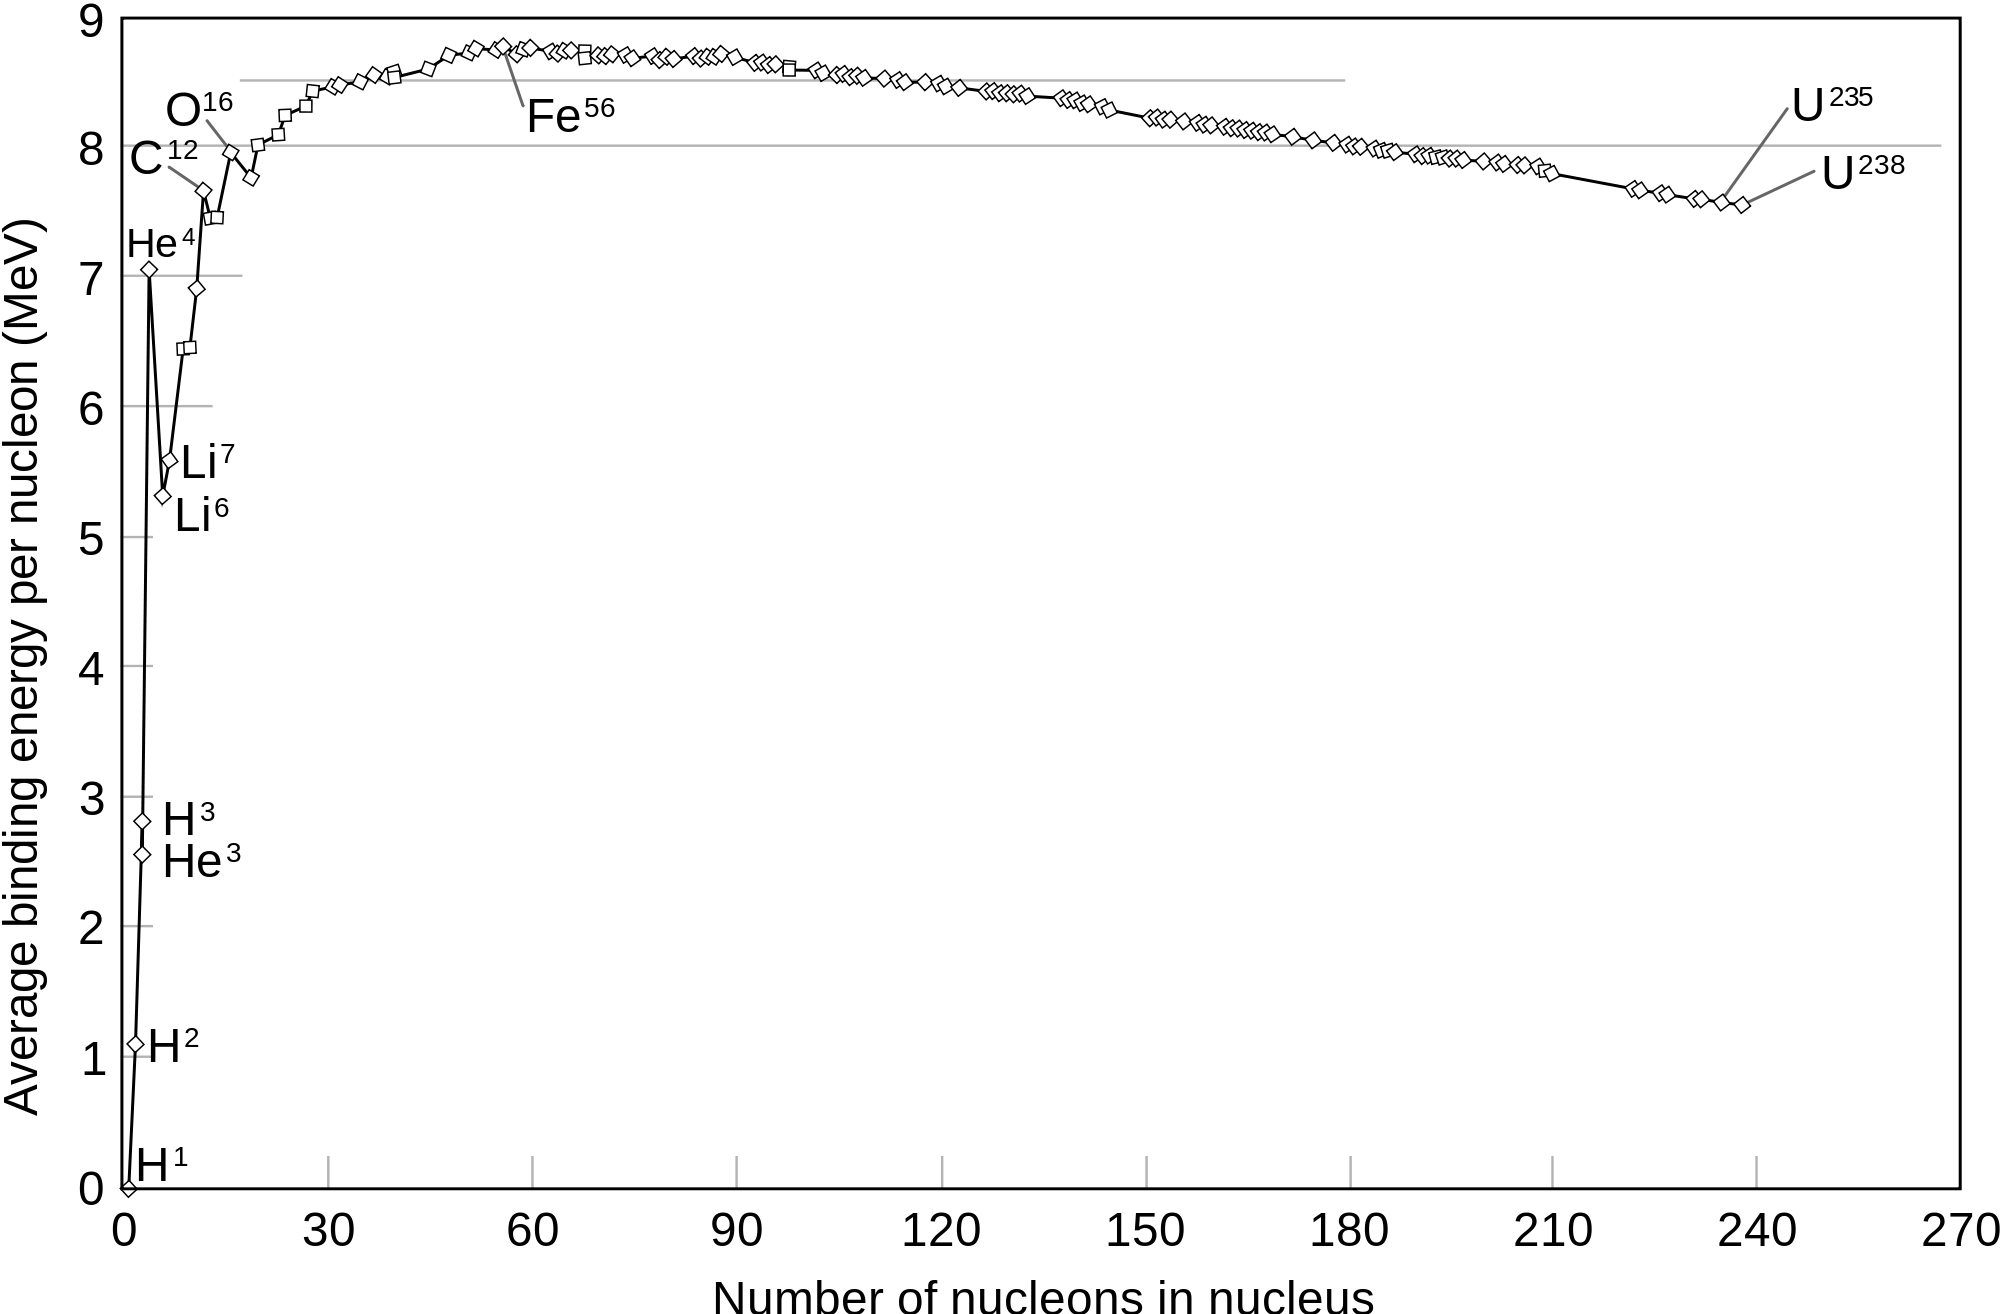
\includegraphics[width=150mm]{graphics/Introduction/bindingenergy.png}}
\end{figure}

\begin{figure}
 \pushtooutside
 \ffigbox[\FBwidth]{\caption[Normalized fusion reaction rate coefficients versus plasma temperature.]{Reaction rate normalized to fuel density, expressed as the rate coefficient $\langle \sigma v \rangle$, for fusion fuels as a function of temperature.  Notably, deuterium-tritium fusion exhibits a higher peak reaction rate, as well as reaching that peak at a lower temperature, than other fuels.}\label{fig:xsection}}{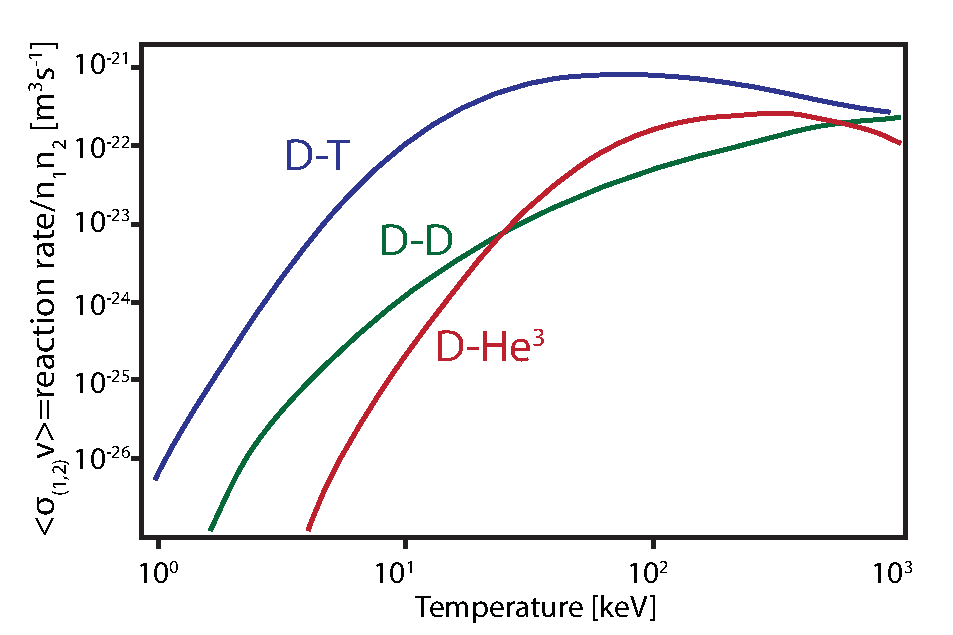
\includegraphics[width=150mm]{graphics/Introduction/reaction_xsections.pdf}}
\end{figure}

Pure deuterium fuel (reactions shown in \cref{eq:dd1,eq:dd2}) is attractive from a research standpoint, due to the abundance and ease of use of deuterium.  Deuterium is a stable nucleus, obviating the need for radiation safety in the fuel system, and is naturally occurring in relative abundance (approximately $1/6420$ of hydrogen nuclei on earth are deuterium \cite{CRC}), allowing harvesting of deuterium fuel from seawater.  However, pure-deuterium reactions suffer from low energy output per reaction and a significantly lower reaction rate at feasible plasma conditions compared to other fuel options (see \cref{fig:xsection}), setting high performance requirements for a putative DD-burning reactor.

The $\si{D}-{}^3\si{He}$ reaction (\cref{eq:dhe3}) exhibits several desirable properties, namely an impressive energy yield per reaction, and the fact that the reaction produces only charged particles rather than the high-energy neutrons found in $\si{D}-\si{D}$ and $\si{D}-\si{T}$ reactions, which can cause significant damage to reactor materials (note, however, that a $\si{D}-{}^3\si{He}$ plasma will also undergo $\si{D}-\si{D}$ fusion, which is neutronic, at a meaningful rate).  However, as with $\si{D}-\si{D}$ fuel, the $\si{D}-{}^3\si{He}$ reaction suffers from a lower reaction rate at attainable conditions, as well as the fact that Helium-3 does not occur in economically usable quantities on Earth.  While off-planet sources of Helium-3 exist (for example, a useful quantity is present in the lunar regolith \cite{Fa2010} and in the atmospheres of some gas giants \cite{Palaszewski2005}), this fuel remains the subject of speculation.

The deuterium-tritium reaction (\cref{eq:dt}) is considered the most promising for a first-generation fusion reactor, due to its high energy output per reaction and favorable reaction cross-section -- the rate parameter $\langle \sigma v \rangle_{DT}$ reaches its peak at a lower temperature, and reaches a greater absolute level than other fusion fuels.  However, $\si{D}-\si{T}$ operation is limited both by fuel sources, and reaction products.  $\si{D}-\si{T}$ fusion produces a $14 \;\si{MeV}$ neutron, carrying roughly 80\% of the energy released by the fusion reaction, which can damage unshielded reactor materials.  Moreover, while deuterium is stable and readily available, tritium is radioactive with a short half-life (roughly 12.3 years), so it is not naturally occurring in meaningful quantities on earth.   A reactor will solve both of these problems with a \emph{neutron blanket}, a neutron-absorbing structure surrounding the plasma.  This provides the necessary shielding for sensitive reactor components.  
The heat generated in the blanket from neutron absorption will also be drawn off in a steam cycle to drive turbines, generating electricity from the reactor.  Finally, seeding the blanket with lithium allows the following reactions with fusion neutrons:

\begin{align}
 {}^6\si{Li} + \si{n}_{slow} &\rightarrow {}^4\si{He} + \si{T} + \SI{4.8}{MeV}\label{eq:Li6}\\
 {}^7\si{Li} + \si{n}_{fast} &\rightarrow {}^4\si{He} + \si{T} + \si{n} - \SI{8.7}{MeV}\label{eq:Li7}
\end{align}

\noindent the Lithium-6 reaction (\cref{eq:Li6}) absorbs ``slow'' neutrons (that is, neutrons that have thermalized to the blanket temperature via collisions) to produce tritium, plus additional heat.  Lithium-7 (\cref{eq:Li7}) is more likely to capture fast neutrons to produce tritium in an endothermic reaction; however, the reaction also acts as a neutron multiplier, as a free neutron is maintained through the reaction.  Using blankets enriched with ${}^6\si{Li}$, coupled with neutron multipliers, a reactor will target an over-unity tritium breeding ratio, with $>1$ tritons produced per neutron entering the blanket (\ie per tritium consumed in a fusion reaction).\nicesectionending

%%%%%%%%%%%%%%%%%%%%%%%%%%%%%%%%%%%%%%%%%%%%%%%%%%%%

\section{Magnetic Confinement}\label{sec:intro_magnetic}

\subsection{Basic Principles}\label{subsec:intro_basic}

The temperatures in excess of 100 million Kelvin necessary for fusion in a plasma are incompatible with any contact between solid reactor materials and the hot core of the plasma.  Magnetic confinement relies on the strong response of the charged particles composing the plasma to magnetic fields, rather than a material wall, to retain the thermal pressure ($\sim 10 \;\si{atm}$ for a reactor) from the plasma.  The response of a charged particle to electric and magnetic fields is governed by the Lorentz force,

\begin{equation}\label{eq:lorentz}
 \vec{F} = q\left(\vec{E} + \vec{v} \times \vec{B}\right)
\end{equation}

\begin{figure}
 \pushtooutside
 \fcapside[50mm]{\caption[Gyro orbits in an applied magnetic field.]{Electron and ion gyro orbits in an applied magnetic field.  Note that, due to the charge dependence in the Lorentz Force (\cref{eq:lorentz}), electrons and ions orbit in opposite directions relative to the magnetic field.}\label{fig:intro_gyro}}{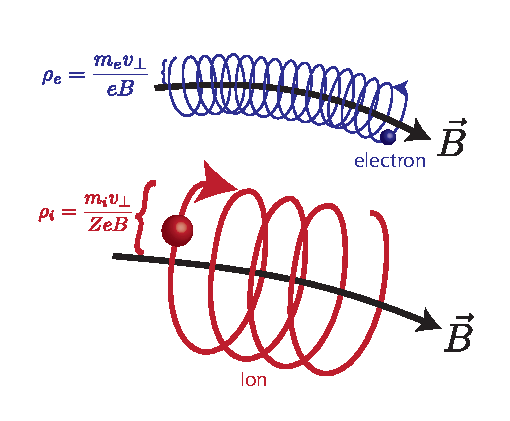
\includegraphics[width=85mm]{graphics/Introduction/gyro.pdf}}
\end{figure}

\noindent In a strong background magnetic field, the particle will move on a helical path along the field line.  The $\vec{v} \times \vec{B}$ factor in the Lorentz Force causes the particle to experience no magnetic force parallel to the field, while velocity perpendicular to the field generates a force proportional to the velocity times the magnetic field, directed perpendicular to both -- thus the particle freely streams parallel to the field, but is trapped in a circular orbit perpendicular to it, termed ``gyro motion'', shown in \cref{fig:intro_gyro}.  The particle will orbit at the cyclotron frequency,

\begin{equation}\label{eq:omegac}
 \omega_c = \frac{qB}{m} \quad\Rightarrow\quad \omega_{ce} = \frac{eB}{m_e}, \quad \omega_{ci} = \frac{ZeB}{m_i}
\end{equation}

\noindent for electrons and ions of charge $Z$, respectively (note that for brevity we indicate the magnitude of vectors as scalar variables, \eg $B = \left|\vec{B}\right|$).  A particle with velocity perpendicular to the magnetic field $v_\perp$ (formally, $v_\perp = \left|\vec{v} \times \vec{B}\right|/B$) orbits at its gyroradius,

\begin{equation}\label{eq:gyroradius}
 \rho = \frac{v_\perp}{\omega_c} = \frac{mv_\perp}{qB}
\end{equation}

\noindent For a thermalized plasma, the perpendicular velocity will, on average, be the thermal velocity $v_t = \sqrt{2T/m}$, thus

\begin{equation}\label{eq:gyroradius2}
 \rho = \frac{\sqrt{2mT}}{qB}
\end{equation}

\noindent The introduction of a nonzero electric field drives additional motion for the particle in the form of a drift velocity -- the guiding center (that is, the average point about which the orbital motion of the particle gyrates) will shift with a bulk velocity (see \cite[\S~8.4]{Freidberg2007} for derivation)

\begin{equation}\label{eq:exb}
 \vec{v}_d = \frac{\vec{E} \times \vec{B}}{B^2}
\end{equation}

\noindent independent of particle charge, mass, or energy.

This restriction of particle motion perpendicular to field lines to short length scales (at fusion-relevant temperatures and magnetic fields, the gyroradius is typically $\sim 10^{-5} \;\si{m}$ for electrons and $\sim 10^{-3} \;\si{m}$ for ions) compared to the size of the plasma is central to the concept of magnetic confinement.  In the perpendicular direction, this scale restriction of particle motion permits a fluid treatment of the dynamics of the plasma.  Further simplification of the fluid model (see \cite[\S~2.3]{Freidberg1987} for detailed derivation) leads to the theory of \emph{magnetohydrodynamics} (MHD), the ``workhorse'' model describing plasma behavior.  A basic equilibrium in a confined plasma is described in MHD by the simple relation

\begin{equation}\label{eq:MHDeq}
 \nabla p = \vec{J} \times \vec{B}
\end{equation}

\noindent in which the outward force due to the plasma pressure gradient is balanced by an inward force from the interplay between magnetic fields and electric currents (expressed by the current density $\vec{J}$).  This interplay is readily illustrated in the simple one-dimensional case of an infinite straight cylinder of plasma -- in this case, the radially-outward $\nabla p$ force may be balanced by an axial current in the $\hat{z}$ direction with an azimuthal $\hat{\theta}$ magnetic field ($z$-pinch), an azimuthal current and axial field ($\theta$-pinch), or a superposition of the two (screw pinch).  However, all three of these options suffer from a lack of parallel confinement -- as the magnetic field does not restrict the free-streaming parallel motion of the plasma, these linear concepts (when reduced to a physical, non-infinite size!) suffer from plasma losses at the ends of the cylinder.  Despite efforts to restrict the parallel motion in a linear device (\eg the \emph{magnetic mirror}, which 
pinches the magnetic field at the cylinder ends in order to reflect the parallel motion of particles with a force due to the field gradient \cite{Kesner1982}), end losses in linear devices proved incompatible with steady-state fusion conditions.  The clear solution, then, was to close the magnetic geometry such that the magnetic field lines have no ends: a \emph{torus.}

\subsection{Toroidal Configurations}\label{subsec:intro_toroidal}

\begin{figure}[h]
 \pushtooutside
 \fcapside[65mm]{\caption[Geometry of a toroidal plasma.]{Example geometry of a circular-cross-section tokamak plasma, describing a torus of major radius $R_0$ and minor radius $a$, with poloidal coordinate $\theta$ and toroidal coordinate $\Phi$.  Tokamak configurations are characterized by an applied toroidal field $B_T$ with a toroidal plasma current $I_p$, which in turn generates a poloidal magnetic field $B_p$.}\label{fig:intro_geometry}}{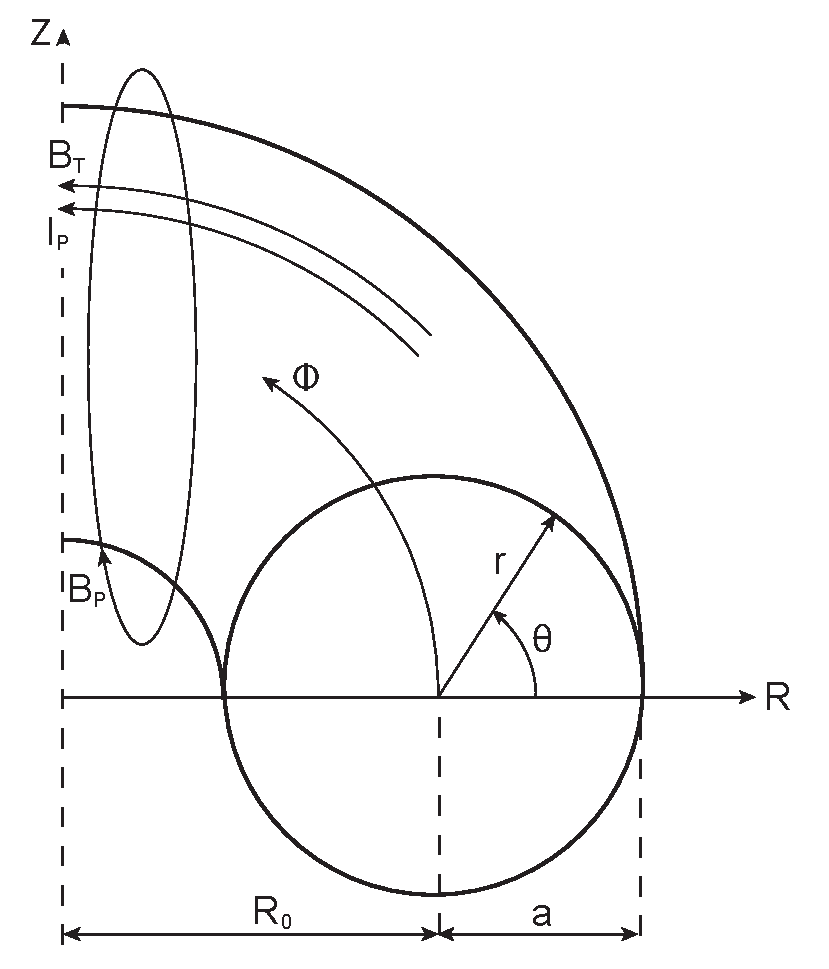
\includegraphics[width=100mm]{graphics/Introduction/geometry.pdf}}
\end{figure}

An example toroidal geometry is shown above in \cref{fig:intro_geometry}.  In comparison to the previous straight cylindrical geometry, the radial coordinate is replaced by a \emph{minor radius} $r$, measured from the center of the plasma column to its edge ($r=a$), while the \emph{major radius} $R_0$ denotes the radius of the torus itself measured from its center axis ($Z$ in \cref{fig:intro_geometry}) to the plasma axis.  The azimuthal cylindrical coordinate is replaced by the poloidal coordinate $\theta$, wrapping immediately about the plasma column.  The axial coordinate in the cylindrical system is replaced by the toroidal angle $\Phi$ wrapping around the center axis of the torus and describing a circuit along the plasma column.  As with the straight cylindrical case, the magnetic geometry may be described with toroidal and poloidal currents and magnetic fields balancing radially-outward thermal pressure.

However, introducing toroidal effects into the magnetic geometry gives rise to additional drift velocities, causing the guiding centers of particle gyro-orbits to shift (see \cite[\S~8.5-7]{Freidberg2007}).  Spatial variation in the magnetic field strength causes the $\nabla B$ drift, given by

\begin{equation}\label{eq:gradbdrift}
 \vec{v}_{\nabla B} = \frac{v_\perp^2}{2\omega_c} \frac{\vec{B} \times \nabla B}{B^2}
\end{equation}

\noindent while the toroidal twist in the magnetic field causes the curvature drift,

\begin{equation}\label{eq:curvaturedrift}
 \vec{v}_\kappa = \frac{v_\parallel^2}{\omega_c} \frac{\vec{R}_c \times \vec{B}}{R_c^2 B}
\end{equation}

\noindent where $v_\parallel$ is the particle velocity parallel to the magnetic field, $\omega_c$ is the species cyclotron frequency (\cref{eq:omegac}), and $\vec{R}_c$ is the radius of curvature of the field.  In the case of an applied toroidal magnetic field, these drifts are directed vertically in the $\hat{Z}$ direction, and are directed oppositely for electrons and ions due to the charge dependence in $\omega_c$.  The electric field resulting from this charge separation drives an outward $\vec{E} \times \vec{B}$ drift (see \cref{eq:exb}), breaking confinement.  This effect is countered by the addition of a poloidal field, which adds a helical twist to the guiding-center path to average out the separation due to particle drifts.  Concepts aiming for steady-state magnetic confinement of a plasma typically rely on generating this twist, termed the \emph{rotational transform}, to maintain stable confinement.
 
One of the most successful implementations of this concept for Magnetic Fusion Energy (MFE) is the \emph{tokamak} \cite{Wesson2011} (a Russian acronym from \foreignlanguage{russian}{тороидальная камера с магнитными катушками}, \emph{toroidalnaya kamera s magnetnymi katushkami}, ``toroidal chamber with magnetic coils'').  The tokamak design is characterized by a strong toroidal magnetic field (variously denoted $B_T$ or $B_\Phi$) applied by external coils, with a poloidal field ($B_p$ or $B_\theta$) primarily generated by a current (termed the \emph{plasma current} $I_p$).  A schematic of the plasma and coil arrangement for a tokamak is shown in \cref{fig:intro_tokamak}.  By generating the rotational transform to the magnetic field using the plasma current, the tokamak design utilizes relatively simple planar magnetic coils, avoiding the significantly more complex three-dimensional coils used to generate the helical field in a \emph{stellarator} (the major competing design concept \cite{Meade2010}).  However, 
the necessity for large ($>\SI{1}{\mega\ampere}$) plasma currents presents a significant engineering and physics challenge.  It is straightforward to generate the plasma current through a simple transformer action from a central solenoid in the torus (depicted in \cref{fig:intro_tokamak}) -- however, this AC-current-driven transformer action necessarily limits tokamaks to pulsed operation.  Generation of non-inductive DC current drive \cite{Westerhof2012}, via RF \cite{Bonoli2014,Prater2004} or particle beams \cite{Gormezano2007}, is an active area of research in tokamak physics and engineering, but is outside the scope of this thesis.

\begin{figure}[t]
 \pushtooutside
 \ffigbox[\FBwidth]{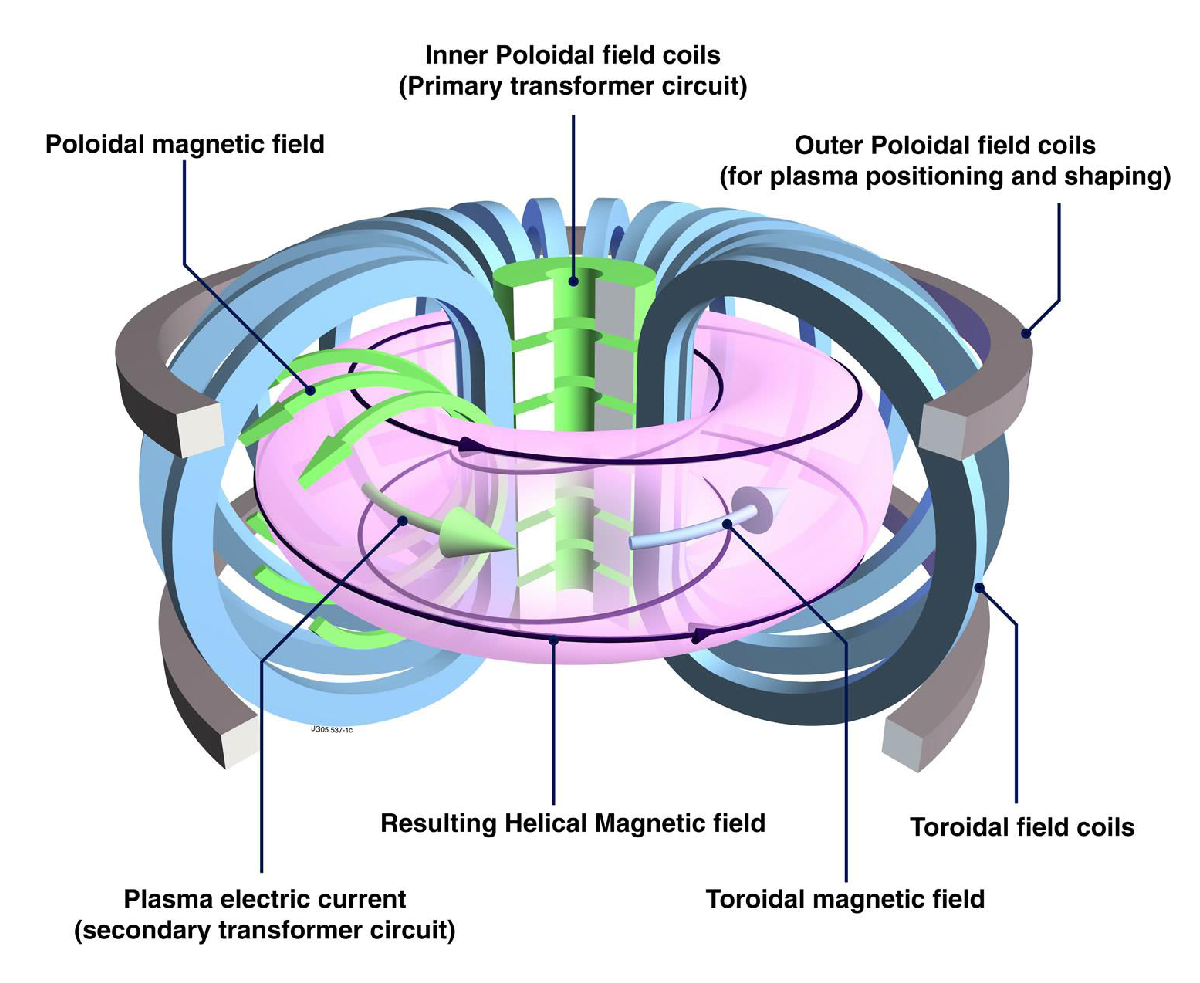
\includegraphics[width=150mm]{graphics/Introduction/tokamak.pdf}}{\caption[Schematic of a tokamak coil configuration and plasma.]{Schematic of a tokamak configuration, showing the plasma and magnetic coils.  The applied toroidal magnetic field is generated by the toroidal field coils (shown in blue).  A toroidal plasma current is generated by the center transformer, in turn generating a poloidal magnetic field (shown in green).  These combine to form the helical magnetic field.  The plasma shape and equilibrium is adjusted with the outer poloidal field coils (gray).}\label{fig:intro_tokamak}}
\end{figure}

Due to its regular, planar magnetic coils and continuous plasma current, tokamak equilibria are characterized by rotational symmetry (to good approximation) about the center axis of the torus (\emph{axisymmetry}).  Solutions to the MHD equilibrium equation, \cref{eq:MHDeq}, thus reduce to a two-dimensional equation in $R$ and $Z$ (as $\partial/\partial \Phi \rightarrow 0$), given by the Grad-Shafranov Equation \cite{Grad1958,Shafranov1960,Freidberg1987}:

\begin{equation}\label{eq:gradshafranov}
 \begin{aligned}
 \Delta^* \psi &= -\mu_0 R^2 \frac{dp}{d\psi} - \frac{1}{2} \frac{dF^2}{d\psi}\\
 \Delta^* \psi &= R^2 \nabla \cdot \left(\frac{1}{R^2} \nabla \psi \right) = R \frac{\partial}{\partial R} \left(\frac{1}{R} \frac{\partial \psi}{\partial R} \right) + \frac{\partial^2 \psi}{\partial Z^2}
 \end{aligned}
\end{equation}

\noindent where $F = RB_\phi$ encodes the toroidal field and $p$ is the thermal pressure.  The poloidal field (equivalently, the plasma current profile) is described by the poloidal magnetic flux $\psi$,

\begin{equation}\label{eq:psi}
 \psi = \frac{1}{2\pi} \int \vec{B}_p \cdot d\vec{S}
\end{equation}

\noindent where $\vec{S}$ is a surface with one edge along the magnetic axis.  In \cref{eq:gradshafranov}, $\psi$ is treated as both an dependent parameter encoding the current, and as an independent variable -- a consequence of Grad-Shafranov is that a number of parameters of interest, including pressure and current density, are \emph{flux functions}, constant on a surface of constant $\psi$, and thus can be expressed as functions of $\psi$ alone, e.g. $p = p(\psi)$.  Moreover, magnetic field lines lie within surfaces of constant flux, with helical structure encoded by the flux function $q(\psi)$, termed the \emph{safety factor}, given for a circular cross-section by

\begin{equation}\label{eq:q}
 q = \frac{rB_\Phi}{RB_\theta}
\end{equation}

\begin{figure}
 \pushtooutside
 \fcapside[55mm]{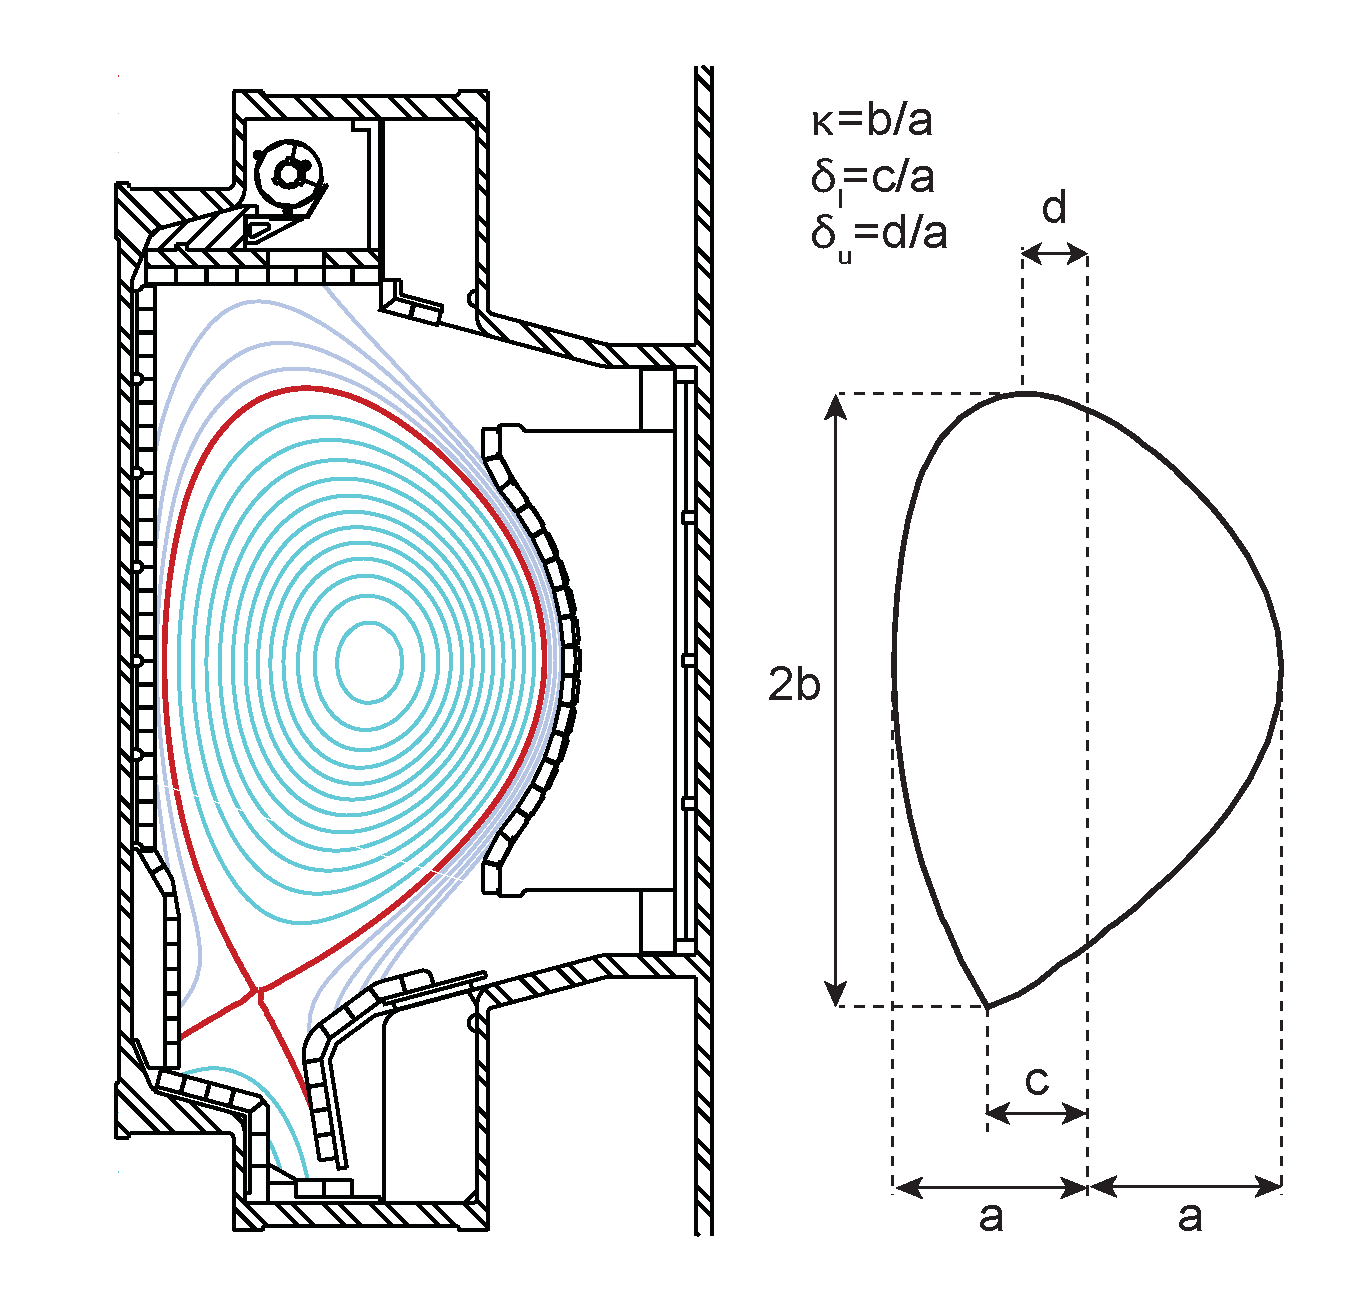
\includegraphics[width=95mm]{graphics/Introduction/shaping.pdf}}{\caption[Tokamak cross-section with shaping parameter definitions.]{Cross-section of a plasma on the Alcator C-Mod tokamak, illustrating closed magnetic flux surfaces (light blue), the last closed flux surface (red), and surfaces with open magnetic field lines (dark blue).  Definitions for plasma shaping parameters elongation $\kappa$, and upper and lower triangularity $\delta_u$, $\delta_l$ are shown at right.}\label{fig:intro_shaping}}
\end{figure}

\noindent As the plasma temperature rapidly equilibrates along field lines, the temperature is also a flux function to good approximation.  It is useful, then, to picture the confined plasma as a series of closed, nested surfaces of constant $\psi$, on which the plasma is trapped (see \cref{fig:intro_shaping}).  In practice, these contours are calculated via a numerical solution of \cref{eq:gradshafranov} by an equilibrium solver such as the EFIT code \cite{Lao1985}.  For flux functions (\ie constant parameters on these flux surfaces), this explicitly removes the dependence on the poloidal angle $\theta$ -- the poloidal flux $\psi$ is thus a useful one-dimensional abscissa derived directly from the magnetic geometry (thus independent of the physical scale of the tokamak and useful for cross-machine comparisons) for the profiles of most parameters of interest, and shall be used thus for the balance of this thesis.

Using outer poloidal field coils (shown in \cref{fig:intro_tokamak}), the tokamak operator may push the plasma into a non-circular shape, with beneficial effects on plasma performance and stability.  In general, flux surfaces sufficiently far from the plasma core will not close on themselves, instead intersecting the wall; the boundary between closed, nested surfaces and these open surfaces is termed the \emph{last closed flux surface} or LCFS.  With sufficient shaping, the operator may generate a null point, the \emph{X-point}, in the LCFS where the poloidal field is zero, splitting the LCFS (also called the \emph{separatrix} in such configurations) into a minimally open surface with ``legs'' contacting the wall.  This magnetic configuration is illustrated in \cref{fig:intro_shaping}, along with a diagram defining the typical plasma shaping parameters: elongation $\kappa$ and upper and lower triangularity $\delta_u$, $\delta_l$.  As the plasma diffuses outwards, it eventually crosses the LCFS and enters 
open flux surfaces in the \emph{scrape-off layer} (SOL).  The plasma then streams freely along these open magnetic field lines until it contacts the wall.  By maintaining an X-point, the operator may steer this plasma exhaust into a section of the tokamak, the \emph{divertor} \cite{Wesson2011}\gnote{find section in Wesson}, that is designed to handle this high heat flux -- a necessary feature to handle reactor-scale exhaust in a tokamak.\nicesectionending

%%%%%%%%%%%%%%%%%%%%%%%%%%%%%%%%%%%%%%%%%%%%%%%%%%%%

\section{Alcator C-Mod}\label{sec:intro_cmod}

\begin{figure}[p]
 \pushtooutside
 \ffigbox[\FBwidth]{\caption[Cutaway view of the Alcator C-Mod tokamk, cryostat and support structure.]{Cutaway view of the Alcator C-Mod tokamak, including cryostat and ancillary structures, illustrating the extensive support structures necessary for compact, high-field operation.}\label{fig:alcator}}{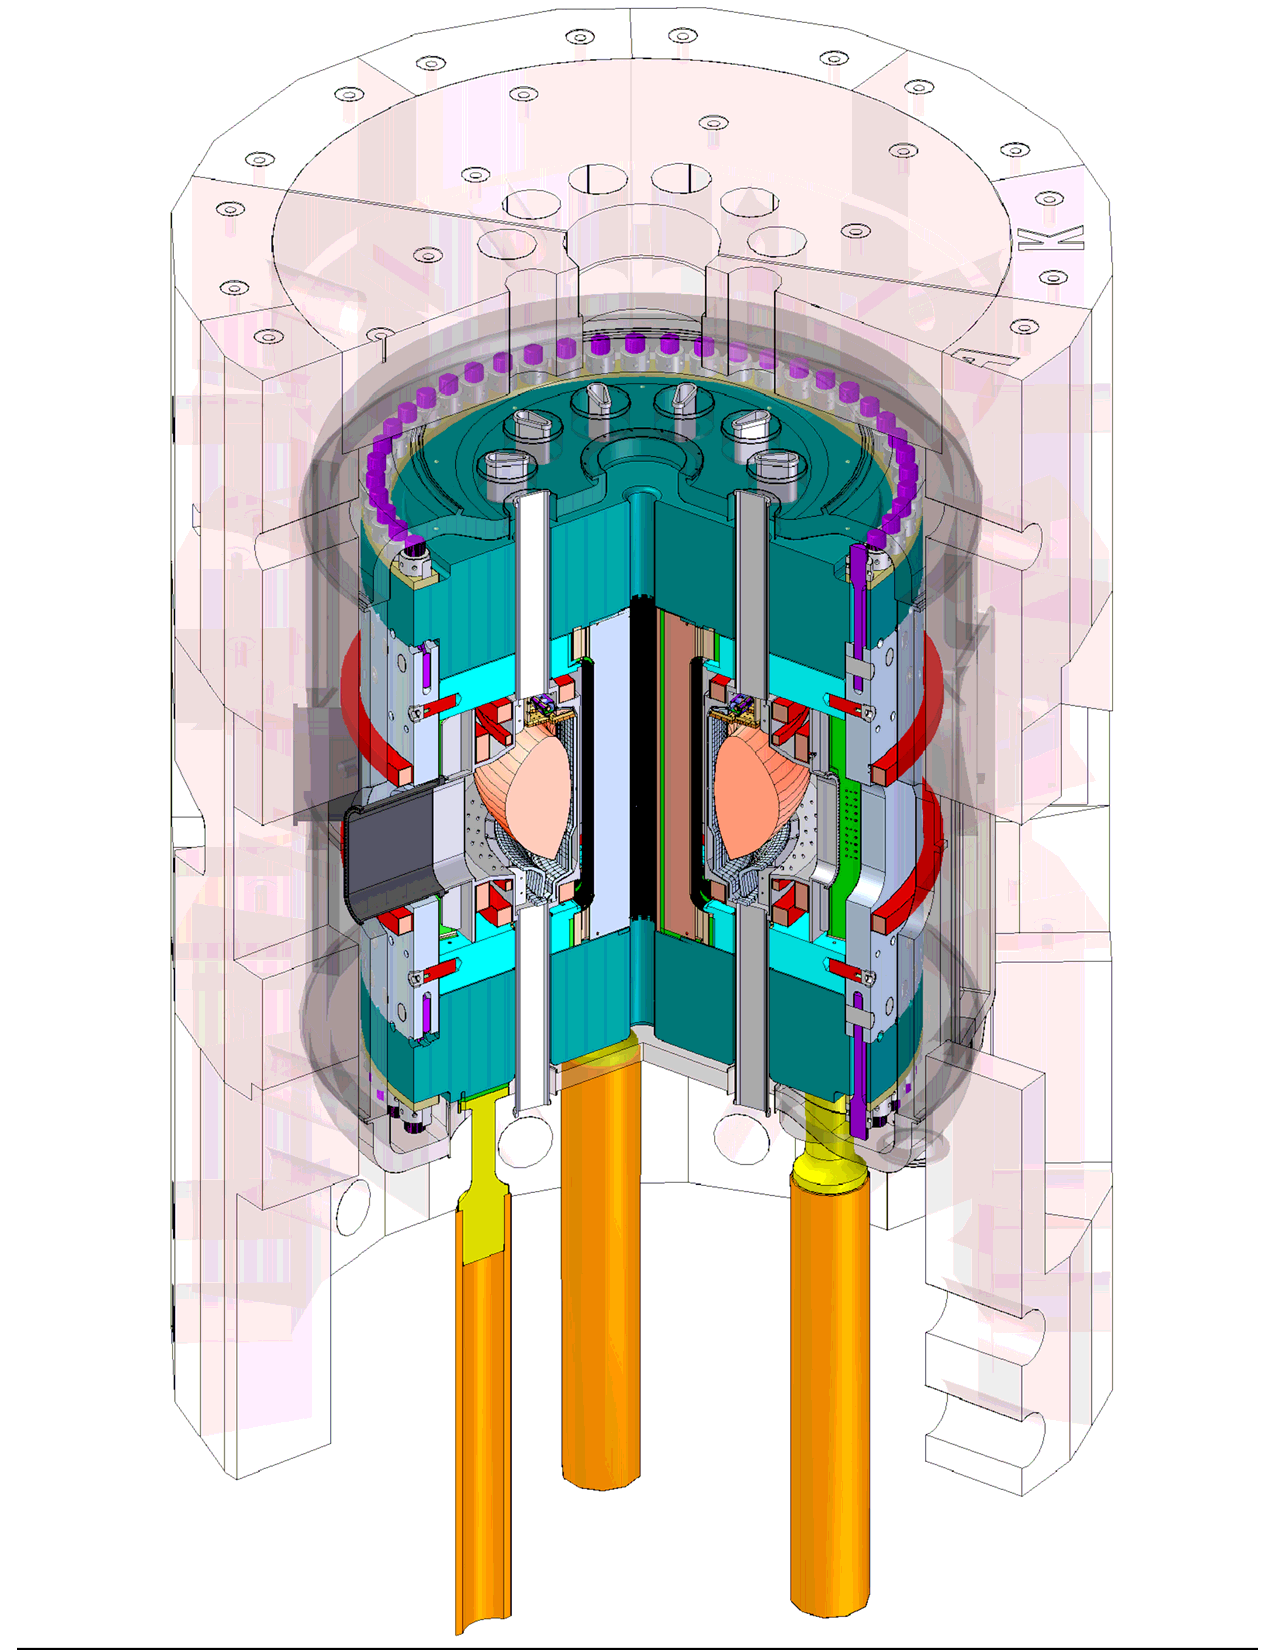
\includegraphics[width=165mm]{graphics/Introduction/alcator.pdf}}
\end{figure}

\begin{wraptable}{O}{0 pt}
 \ttabbox{\caption{Summary of Alcator C-Mod typical operating parameters.}\label{tab:cmod}}
  {\begin{tabular}{lc}
    \toprule
    \emph{parameter} & \emph{range}\\
    \midrule
    major radius & $\SI{0.67}{\meter}$ \\
    minor radius & $\SI{0.22}{\meter}$ \\
    toroidal field & $3 - \SI{8.1}{\tesla}$ \\
    plasma current & $\le \SI{2}{\mega\ampere}$ \\
    plasma density & $\le \SI{5e20}{m^{-3}}$ \\
    central temperature & $\le \SI{8}{\kilo\electronvolt}$ \\
    plasma pressure & $\le \SI{2}{\atmosphere}$ \\
    ICRF power & $\SI{6}{\mega\watt}$ \\
    LHRF power & $\SI{1}{\mega\watt}$ \\
    \bottomrule
   \end{tabular}}
\end{wraptable}

The data presented in this thesis were collected on the Alcator C-Mod tokamak \cite{Hutchinson1994,Greenwald2007} at the MIT Plasma Science and Fusion Center.  The Alcator series of tokamak experiments were designed as compact, high-field tokamaks.  Despite its small physical size ($\SI{67}{\centi\meter}$ major radius, $\SI{22}{\centi\meter}$ minor radius, considerably smaller than other major experiments), Alcator C-Mod plasmas are capable of reaching ITER- and reactor-relevant densities ($> \SI{1e20}{m^{-3}}$) and pressures ($>\SI{1}{\atmosphere}$).  This compact design is enabled by a very high toroidal magnetic field driven by liquid-Nitrogen-cooled copper coils, reaching as high as $\SI{8.1}{\tesla}$, with typical operation near $\SI{5.5}{\tesla}$, allowing reactor-relevant research in a small, cost-effective machine.  C-Mod plasmas are primarily heated by ion-cyclotron (ICRF) heating \cite{Takase1996}, with up to $\SI{6}{\mega\watt}$ of heating power, with an additional $\sim \SI{1}{\mega\watt}$ of 
lower-hybrid resonance (LHRF) power used for heating and DC current drive \cite{Wilson2009}, providing exceptionally high power density in the $\sim \SI{1.1}{\meter\cubed}$ plasma.  A cutaway view of C-Mod, including support structures and the concrete ``igloo'' housing the cooling systems, is visible in \cref{fig:alcator}.  A detailed and annotated view of the C-Mod cross-section is shown in \cref{fig:alcator2}.

\begin{figure}[t]
 \pushtooutside
 \ffigbox[\FBwidth]{\caption[Labeled cross-section of the C-Mod vacuum vessel.]{Cross-section of the C-Mod vacuum vessel, cryostat and diagnostic access ports, with toroidal-field and equilibrium-field magnetic coils labeled.  Also shown is the plasma position in a typical LSN shape, with strike points in the lower divertor shown..}\label{fig:alcator2}}{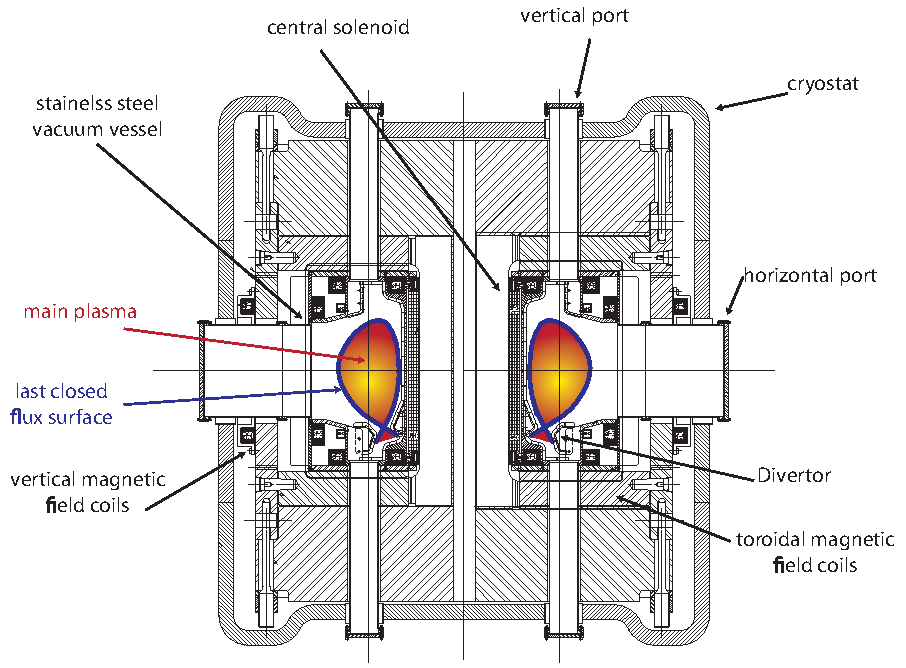
\includegraphics[width=150mm]{graphics/Introduction/cmod_xsec.pdf}}
\end{figure}

Due to their high plasma pressure and power density, C-Mod plasmas must exhaust a large heat flux, reaching levels comparable to that anticipated for ITER \cite{Loarte2007,Terry2007,LaBombard2011}.  To handle this heat flux, C-Mod operates entirely with high-$Z$ metal materials (primarily Molybdenum and Tungsten) for all plasma-facing surfaces.  In addition to its high heat tolerance and low erosion rates due to plasma contact, metal walls provide low retention of fuel gas at the edge -- metal walls are thus the leading candidate for ITER- and reactor-scale plasma-facing components.

The presence of a full high-$Z$ lower divertor and upper strike plate, as well as metal limiter walls, gives C-Mod great flexibility in attainable plasma shapes -- plasmas may be run in a lower-single null (LSN) shape with the plasma exhaust striking the lower divertor (shown in \cref{fig:alcator2}, upper-single null (USN) exhausting into the upper strike plate, or in a limited shape where the scrape-off layer directly impinges on the plasma-facing wall.\nicesectionending

%%%%%%%%%%%%%%%%%%%%%%%%%%%%%%%%%%%%%%%%%%%%%%%%%%%%

\section{Confinement \& Transport}\label{sec:intro_confinement}

\subsection{Global Confinement}\label{subsec:intro_global}

The rate at which a fusion plasma bleeds off heat is described by a characteristic time scale, the energy confinement time $\tau_E$.  From basic power balance for the total plasma stored energy $W_p$,

\begin{equation}\label{eq:powerbalance}
 \frac{dW_p}{dt} = P_{in} - P_{out} = P_{in} - P_{rad} - \frac{W_p}{\tau_E}
\end{equation}

\noindent where $P_{in}$ is input heating power, from Ohmic heating $P_{Ohm} = I_p^2 R_{plasma}$, RF or beam auxiliary heating power $P_{aux}$, or self-heating of the plasma from fusion reactions.  In the case of the latter, note that as fusion neutrons are immediately lost into the blanket, only the energy carried by \emph{charged} fusion products contributes to fusion self-heating: in the case of $\si{D} - \si{T}$ fusion we denote this as the alpha heating power $P_{\alpha} = 1/5 \times P_{fusion}$ for the energy carried by the ${}^4\si{He}$ nucleus.  $P_{rad}$ denotes the power loss due to radiative (primarily, Bremsstrahlung) effects, which are considered separately from the transport-driven heat losses encoded by $W_p/\tau_E$.  It is common to encapsulate these heat source and sink terms into a single net power,

\begin{equation}\label{eq:pnet}
 P_{net} = P_{Ohm} + P_{aux} + P_{fusion} - P_{rad} - \frac{dW_p}{dt}
\end{equation}

\noindent The radiative power loss is occasionally difficult to consistently determine experimentally, is in any case largely independent of operator control (as in the case of auxiliary heating power, or Ohmic power determined by the choice of plasma current) or bulk plasma performance (as in the suppression of turbulent heat losses in high-performance operation), and is relatively negligible at fusion conditions due to its weak scaling with temperature.  As such, it is alternately common to express the power as

\begin{equation}\label{eq:ploss}
 \begin{aligned}
 P_{loss} &= P_{Ohm} + P_{aux} + P_{fusion} - \frac{dW_p}{dt} \\
 P_{net} &= P_{loss} - P_{rad}
 \end{aligned}
\end{equation}

\noindent These definitions allow a simple relation for the experimental energy confinement time,

\begin{equation}\label{eq:tauE}
 \tau_E = \frac{W_p}{P_{net}}
\end{equation}

\noindent In practice, the physics determining energy confinement are extremely complex; as such, working models for calculating $\tau_E$ from bulk parameters typically require an empirical power-law scaling.

A closer examination of the power balance equation, \cref{eq:powerbalance}, reveals an important figure of merit.  For a DT-burning fusion reactor, steady-state operation with plasma temperatures sustained by fusion self-heating (termed ``ignition'') is highly desirable.  At these conditions, Bremsstrahlung losses are small, so \cref{eq:powerbalance} reduces to simply

\begin{equation}\label{eq:powerbalance2}
 \frac{W_p}{\tau_E} = P_{\alpha}
\end{equation}

\noindent The alpha heating power is simply the fusion reaction rate $R_f = n_D n_T \langle \sigma v \rangle_{DT}$ times the energy carried by charged particles from a single reaction, $E_\alpha = 1/5 \times E_{fusion} = \SI{3.5}{\mega\electronvolt}$.  Quasineutrality (\cref{eq:quasineutral}) requires $n_e \approx n_D + n_T$.  As the reaction rate is optimized for a 50-50 fuel mix, the alpha heating power is given by

\begin{equation}\label{eq:palpha}
 P_{\alpha} = \frac{1}{4} n_e^2 \langle \sigma v \rangle E_\alpha
\end{equation}

\noindent The stored energy is defined by

\begin{equation}\label{eq:Wp}
 W_p = \frac{3}{2}p_{thermal}
\end{equation}

\noindent with the thermal pressure in the plasma given by

\begin{equation}\label{eq:pthermal}
 p_{thermal} = n_e T_e + n_D T_D + n_T T_T = 2 n_e T_e
\end{equation}

\noindent assuming the condition above on the electron and ion densities, and assuming temperature equilibration $T_e \approx T_D \approx T_T$.  This, then, implies $W_p = 3 n_e T_e$ (a convenient expression, as electron quantities are typically more readily measured in plasma experiments).  Power balance at ignition then requires

\begin{equation}\label{powerbalance3}
 \frac{3n_e T_e}{\tau_E} = \frac{1}{4} n_e^2 \langle \sigma v \rangle E_\alpha
\end{equation}

\noindent thus simplifying to the Lawson Criterion \cite{Lawson1957}

\begin{equation}\label{eq:lawson}
 n_e \tau_E = \frac{12 T_e}{\langle \sigma v \rangle E_\alpha}
\end{equation}

\noindent Scaling both sides by $2T_e$ gives the ``triple product,''

\begin{equation}\label{eq:tripleproduct}
 2 n_e T_e \tau_E = p \tau_E = \frac{24 T_e^2}{\langle \sigma v \rangle E_\alpha}
\end{equation}

\noindent an important figure of merit for a reactor that is optimized at $T_e \approx \SI{15}{\kilo\electronvolt}$ with a value of $p \tau_E \approx \SI{8.3}{\atmosphere\cdot\second}$, setting target parameters for a fusion reactor \cite{Meade2010}.

However, the maximum attainable thermal pressure in a tokamak is limited by a global MHD stability limit expressed in terms of the normalized pressure \cite[\S~6.16]{Wesson2011}

\begin{equation}\label{eq:beta}
 \beta = \frac{2 \mu_0 p}{B^2}
\end{equation}

\noindent which encodes the ratio of thermal pressure to magnetic pressure $B^2/2\mu_0$ (equivalently, the ratio of thermal and magnetic stored energy) -- a normalization that also falls naturally out of solutions to the MHD equilibrium, \cref{eq:MHDeq}.  Although the maximum stable pressure may be increased with higher plasma current and toroidal field (motivating high-field design for tokamaks), reactor-scale operation requires increased energy confinement -- that is, higher values for $\tau_E$ -- to reach the triple-product target.

\subsection{Transport Barriers}\label{subsec:intro_barriers}

Global improvement to energy confinement may be achieved through local modification of the transport of energy or particles out of the plasma, achieved via structures termed \emph{transport barriers}.  While the physics driving the formation of transport barriers is not entirely understood\gnote{how deep to go with this?}, the effect is evidently caused by sheared flows in the plasma -- these break up the turbulent ``eddies'' driving much of the energy or particle transport through the plasma, locally reducing transport drive in the sheared region.  

The effect on the transport is clearly evident from a diffusive transport model, given by

\begin{equation}\label{eq:diffusion}
 \frac{\partial Q}{\partial t} = \nabla \cdot \left( D_Q \nabla Q \right) + R_Q
\end{equation}

\noindent for a general parameter $Q(\vec{x},t)$ with accompanying diffusion coefficient $D_Q(Q,\vec{x},t)$ and net source/sink term $R_Q(Q,\vec{x},t)$.  We may consider a one-dimensional ``toy model'' of diffusion with a simple constant source term, given in steady state by

\begin{equation}\label{eq:diffusion2}
 \frac{d}{dx} \left( D_Q \frac{dQ}{dx} \right) + R_Q = 0
\end{equation}

 \begin{wrapfigure}{O}[\marginparwidth+\marginparsep]{70mm}
  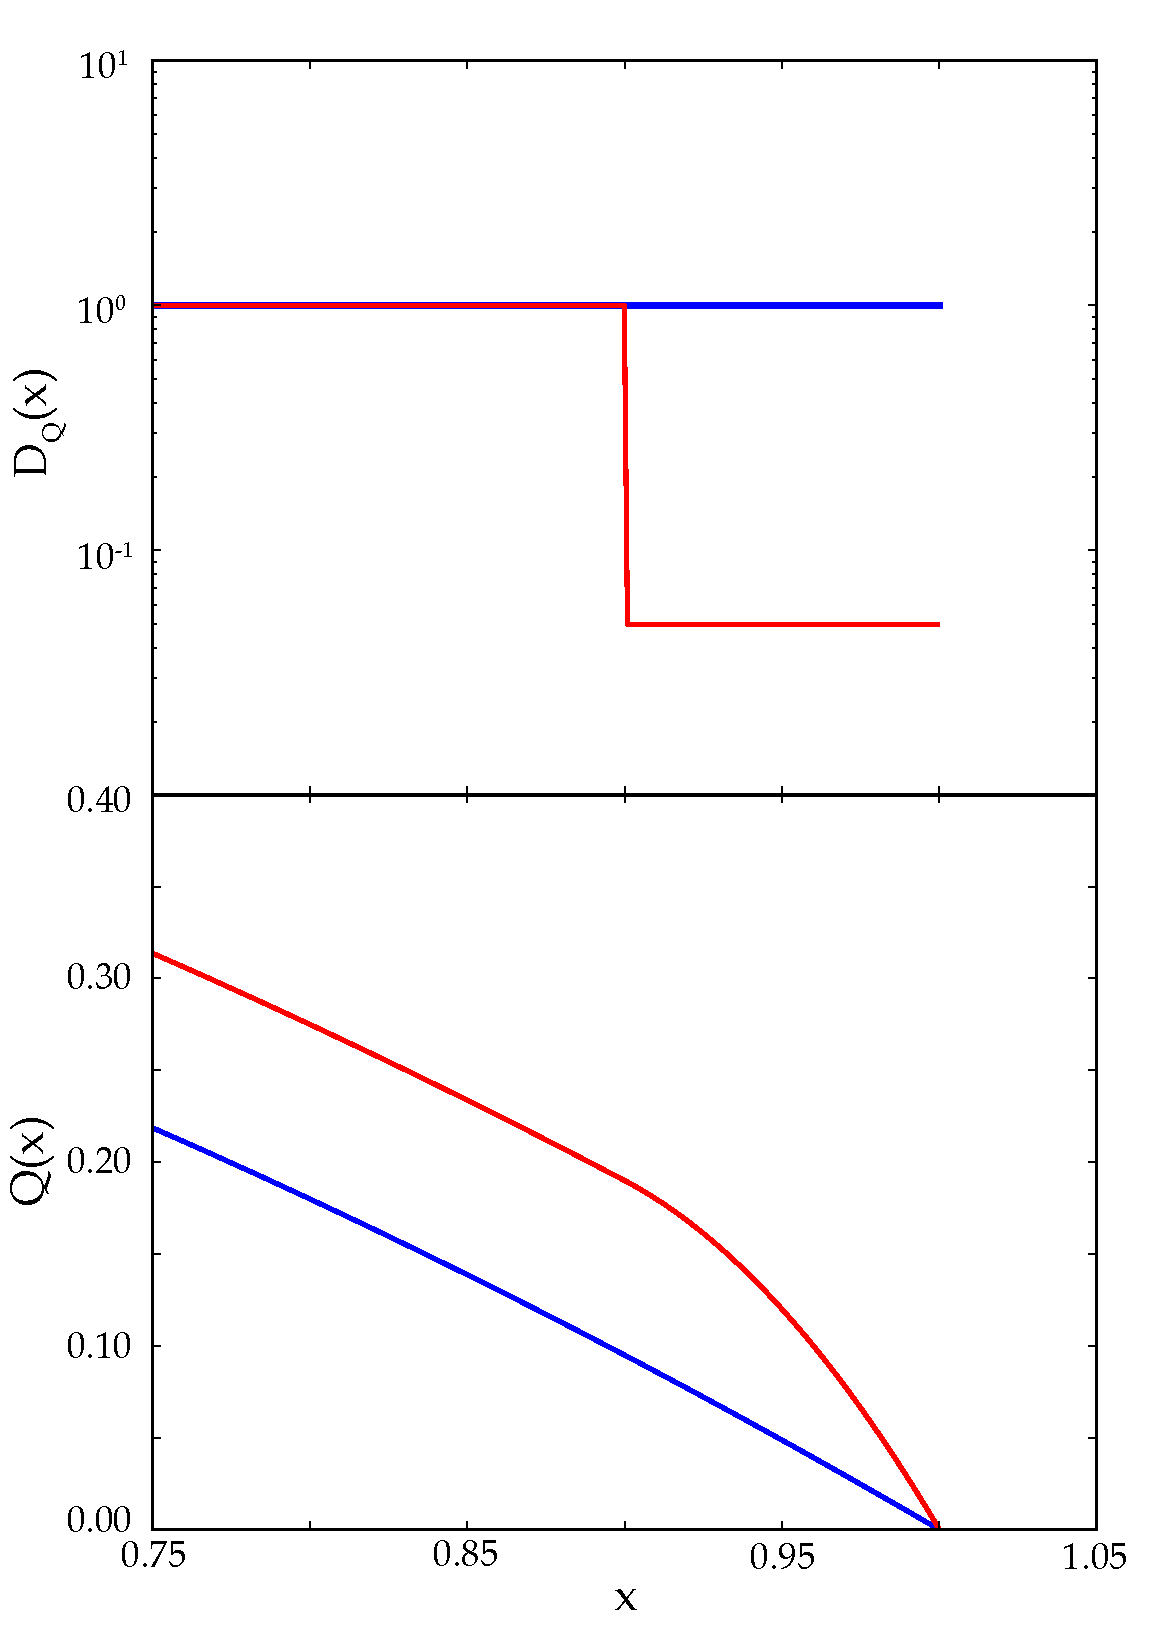
\includegraphics[width=70mm]{graphics/Introduction/transport.pdf}
  \caption[Diffusion coefficients and plasma profiles for a ``toy model'' diffusion equation.]{Diffusion coefficients and plasma profiles for a ``toy model'' 1D diffusion equation with a general parameter $Q(x)$ and accompanying diffusion coefficient $D_Q(x)$.}
  \label{fig:intro_transport}
 \end{wrapfigure}

\noindent The solution to this model for two sample diffusion coefficients is given in \cref{fig:intro_transport}.  A simple constant diffusion coefficient $D_Q$ produces a profile with weak slope, whereas an order-of-magnitude drop in $D_Q$ near the edge (consistent with experimentally-observed values of diffusion coefficients in transport barriers) produces a region with a steep gradient in $Q$ compared to the flat-$D_Q$ solution, despite identical source terms $R_Q$.  Experimentally, reductions in the particle transport coefficient $D_n$ or the heat transport coefficient $\chi$ due to sheared flows correspond to steep-gradient regions in density or temperature, characteristic of the transport barrier.

Of particular interest is the \emph{edge transport barrier}, also termed the \emph{pedestal} \cite{Wagner1982,Greenwald1997}.  A number of high-performance tokamak regimes have been established, exploiting the formation of a pedestal to suppress transport and boost global energy confinement to levels necessary to reach the triple-product target (\cref{eq:tripleproduct}) for an ignited plasma.  The understanding of these high-performance regimes, commonly referred to as ``high-confinement'' or H-modes, and their extrapolation to ITER and reactor-scale devices has been a major focus of recent tokamak research.

However, the formation of the pedestal also presents challenges that must be addressed for reactor-scale operation.  Increased particle confinement causes the plasma to retain impurities -- particularly ionized wall materials -- along with fuel ions.  These impurities both dilute the fuel, slowing the fusion reaction rate\gnote{show equation for this?}, and drive elevated radiative losses due to their higher nuclear charge (note the strong charge dependence in \cref{eq:brems}).  This ultimately leads to a \emph{radiative collapse}\gnote{cite for this?}, dropping the plasma out of H-mode -- thus, stationary (\ie non-transient) operation in H-mode requires a means to regulate particle confinement and flush impurities from the plasma core.  

The steep gradient in the plasma pressure generated in the pedestal has been shown to drive \emph{Edge-Localized Modes} (ELMs) \cite{Zohm1996}\gnote{more cites?}, instabilities that cause the pedestal to periodically ``crash,'' expelling particles and energy into the scrape-off layer.  The smaller ELM bursts found in existing experiments provide the desired level of particle transport for stationary operation -- thus ITER operation is designed considering an H-mode with ELMs as the baseline for operation \cite{ITER1999,Shimada2007}.  However, on ITER-scale devices the heat pulses from ELMs drive unacceptable levels of transient thermal loading and erosion damage to wall and divertor materials \cite{Loarte2003,Federici2003}.  As such, high-performance operation on ITER- or reactor-scale devices requires mitigation or elimination of large, deleterious ELMs, either through externally-applied controls or physics-based stabilization.\nicesectionending

%%%%%%%%%%%%%%%%%%%%%%%%%%%%%%%%%%%%%%%%%%%%%%%%%%%%

\section{Goals \& Outline}\label{sec:intro_outline}

This thesis will present results in the \emph{I-mode}, a novel high-performance regime pioneered on Alcator C-Mod.  I-mode is notable for its apparent decoupling of energy and particle transport, reaching H-mode-like energy confinement while maintaining L-mode levels of particle and impurity transport, achieving the desired flushing of impurities from the plasma.  This manifests in the edge with the formation of an H-mode-like temperature pedestal without the accompanying density pedestal found in conventional H-modes.  I-mode also appears to be naturally free of large ELMs, avoiding the need for complex externally-applied controls, and to exhibit highly favorable scalings of energy confinement with heating power.

A firm understanding of the structure and stability of the pedestal is essential to extend I-mode operation to larger devices.  This thesis will describe a combined approach to the understanding of the pedestal in I-mode, using both direct observations of pedestal structure and numerical modeling of the pedestal stability against identified triggers for large, deleterious ELMs, to better establish the operating space and reliability of I-mode for reactor operation.\gnote{reword this}  The balance of the thesis is arranged as follows:

\begin{description}
 \item[Chapter \ref{ch:HighPerformance}: High-Performance Regimes] \hfill \\
 An overview of of existing results in established H-mode regimes, including observed pedestal behaviors.  A detailed introduction to I-mode physics and operation is also included.
 \item[Chapter \ref{ch:Modeling}: Pedestal Modeling and Theory] \hfill \\
 An introduction to the theory of the MHD and turbulent instabilities governing the pedestal and driving large ELMs, and the numerical modeling approaches used in their analysis.
 \item[Chapter \ref{ch:Elmy}: ELMy H-Modes on C-Mod] \hfill \\
 The results of recent experiments on C-Mod testing a unified model for pedestal structure in ELMy H-mode, the approach to which is also applied to I-mode pedestals.
 \item[Chapter \ref{ch:ImodePedestal}: I-Mode Pedestal Scalings] \hfill \\
 New results from dedicated pedestal experiments in I-mode examining the response of pedestal structure to engineering and physics parameters, and potential extrapolations of pedestal structure and performance to larger devices.
 \item[Chapter \ref{ch:ImodeModeling}: I-Mode Pedestal Stability Modeling] \hfill \\
 Numerical modeling results for the stability of I-mode pedestals against identified ELM triggers, and correlations to the generally observed lack of ELMs in I-mode.
 \item[Chapter \ref{ch:Conclusion}: Conclusions] \hfill \\
 A summary of the results presented in this thesis and some directions for future work.
\end{description}

\noindent An overview of the diagnostics used in the experiments presented here is also given in \cref{app:Diagnostics}.  A summary of the pedestal database used in these experiments is given in \cref{app:sql}.\nicechapterending

%%%%%%%%%%%%%%%%%%%%%%%%%%%%%%%%%%%%%%%%%%%%%%%%%%%%

% do per-chapter bibliographies, or one big one?
\bibliographystyle{../plainurl}
\bibliography{../references} 
\cleardoublepage
% ********************************************************************
% Backmatter
%*******************************************************
\appendix
\cleardoublepage
%%\part{Appendix}
%\cleardoublepage\include{FrontBackmatter/sheath_heat_flux_derivation}
%********************************************************************
% Other Stuff in the Back
\cleardoublepage\bibliographystyle{plainurl}
\bibliography{references}
%*******************************************************\bigwedge
\cleardoublepage\pagestyle{empty}

\hfill

\vfill


\pdfbookmark[0]{Colophon}{colophon}
\section*{Colophon}
This document was typeset using \texttt{classicthesis} developed by Andr\'e Miede (although aspects were changed to comply with the MIT thesis standards and the author's personal preferences).
The style was inspired by Robert Bringhurst's seminal book on typography ``\emph{The Elements of Typographic Style}''.
\texttt{classicthesis} is available for both \LaTeX\ and \mLyX:
\begin{center}
\url{http://code.google.com/p/classicthesis/}
\end{center}

\bigskip

\noindent\finalVersionString

Hermann Zapf's \emph{Palatino} and \emph{Euler} type faces (Type~1 PostScript fonts \emph{URW
Palladio L} and \emph{FPL}) are used. The ``typewriter'' text is typeset in \emph{FPL},
originally developed by Bitstream, Inc. as ``Bitstream Vera''. (Type~1 PostScript fonts were made available by Malte Rosenau and Ulrich Dirr.)

%\paragraph{note:} The custom size of the textblock was calculated
%using the directions given by Mr. Bringhurst (pages 26--29 and
%175/176). 10~pt Palatino needs  133.21~pt for the string
%``abcdefghijklmnopqrstuvwxyz''. This yields a good line length between
%24--26~pc (288--312~pt). Using a ``\emph{double square textblock}''
%with a 1:2 ratio this results in a textblock of 312:624~pt (which
%includes the headline in this design). A good alternative would be the
%``\emph{golden section textblock}'' with a ratio of 1:1.62, here
%312:505.44~pt. For comparison, \texttt{DIV9} of the \texttt{typearea}
%package results in a line length of 389~pt (32.4~pc), which is by far
%too long. However, this information will only be of interest for
%hardcore pseudo-typographers like me.%
%
%To make your own calculations, use the following commands and look up
%the corresponding lengths in the book:
%\begin{verbatim}
%    \settowidth{\abcd}{abcdefghijklmnopqrstuvwxyz}
%    \the\abcd\ % prints the value of the length
%\end{verbatim}
%Please see the file \texttt{classicthesis.sty} for some precalculated
%values for Palatino and Minion.
%
%    \settowidth{\abcd}{abcdefghijklmnopqrstuvwxyz}
%    \the\abcd\ % prints the value of the length





% ********************************************************************
\end{document}
% ********************************************************************
